\documentclass{article}
\usepackage[utf8]{inputenc}
\usepackage{geometry}[margins = 1in]
\usepackage{graphicx}
\usepackage{hyperref}
\usepackage{eufrak}
\usepackage{fullpage}
\usepackage{physics}
\usepackage{amsmath}
\usepackage{listings}
\usepackage[makeroom]{cancel}
\usepackage{color}
\usepackage{amssymb}
\usepackage{float}
\floatplacement{figure}{H}
\setkeys{Gin}{width=0.75\linewidth}

\hypersetup{
    colorlinks=true, %set true if you want colored links
    linktoc=all,     %set to all if you want both sections and subsections linked
    linkcolor=blue,  %choose some color if you want links to stand out
}


\newcommand{\unit}[1]{{\,\rm #1}}
\newcommand{\be}{\begin{equation}}
\newcommand{\ee}{\end{equation}}
\newcommand{\Mpc}{\unit{Mpc}}
\newcommand{\Gpc}{\unit{Gpc}}
\newcommand{\Gyr}{\unit{Gyr}}
\newcommand{\s}{\unit{s}}
\newcommand{\km}{\unit{km}}
\newcommand{\yr}{\unit{yr}}
\newcommand{\g}{\unit{g}}
\newcommand{\cm}{\unit{cm}}
\newcommand{\frw}{\mathrm{d}s^2 = c^2 \mathrm{d}t^2 - a^2\left(t\right) \left[\frac{\mathrm{d}r^2}{1-kr^2} + r^2 \left(\mathrm{d}\theta^2 + \sin^2\theta \mathrm{d}\phi^2\right) \right]}


%%%%%
\def\:{\ddot }
\def\.{\dot }
\def\^{\hat }
\def\_{\bar }
\def\~{\tilde }
\def\hf{\frac12}
\def\imply{\Rightarrow}
\def\inv#1{\frac{1}{ #1}}
\def\ddt{\frac{d}{dt}}
\def\aa{\frac{\dot a }{ a}}
\def\adda{\frac{\ddot a}{ a}}
\def\thnot{\theta_0}
\def\etot{\Omega_0}
\def\econs{\Omega_{0,\Lambda}}
\def\emat{\Omega_{0,M}}
\def\econs{\Omega_{0,\Lambda}}
\def\p{^\prime}
\def\iff{\Leftrightarrow}
\def\xv{{\vec x}}
\def\pv{{\vec p}}
\def\vv{{\vec v}}
\def\ppt{\frac{\partial}{\partial t}}
\def\ddt{\frac{d}{dt}}
\def\epot{\frac{8\pi}{ 3}}
\def\attw{a^{3+3w}}
\def\athow{a^{-\frac{3}{2}(1+w)}}
\def\atow{a^{-3(1+w)}}
\def\atowi{a^{-3(1+w_i)}}
\def\hf{\frac12}
\def\imply{\Rightarrow}
\def\thnot{\theta_0}
\def\etot{\Omega_0}
\def\econs{\Omega_{0,\Lambda}}
\def\emat{\Omega_{0,M}}
\def\econs{\Omega_{0,\Lambda}}
\def\p{^\prime}
\def\iff{\Leftrightarrow}
\def\xv{{\vec x}}\def\pv{{\vec p}}
\def\vv{{\vec v}}
\def\ddt{{\frac{d}{dt}}}
\def\atow{a^{-3(1+w)}}
\def\atowi{a^{-3(1+w_i)}}
\def\attw{a^{3+3w}}
\def\cc{Cosmological constant}
\def\jumble{\frac{\Omega _0}{ \attw} + \frac{1 - \Omega _0}{ a^2}}
\def\jimble{\sqrt{\Omega _{0,m}(1+z)^3+\Omega _{0,\Lambda}+(1-\Omega _{0,m}-\Omega _{0,\Lambda})(1+z)^2}}
\def\paap{\left(\aa\right)}
\def\rcr{{\rho_{crit}}}




\title{Extragalactic Astrophysics and Comsology}
\author{Jacob Pilawa}
\date{Spring 2021}

\begin{document}

\maketitle
\tableofcontents
\newpage

\section{The Smooth Universe}
\subsection{The Cosmological Principle; The Hubble Parameter; Scale Factor}

\subsubsection{The Cosmological Principle}

We begin with \textbf{The cosmological Principle}. It sounds simple, but incredibly well supported. It says that \textbf{the Universe (spatially) is homogeneous and isotropic on very large spatial scales}. Observationally, this is around $100 \Mpc$ scales. Homogeneous means constant density (non-realistically, this is mass density; relativistic ally, this is energy density). Isotropic means the same in all directions. 

\textit{Note}: Isotropy about $2$ points (or more) implies homogeneity. Isotropy about $1$ point is not enough. Here is a quick illustration of that: 

\begin{figure}
    \centering
    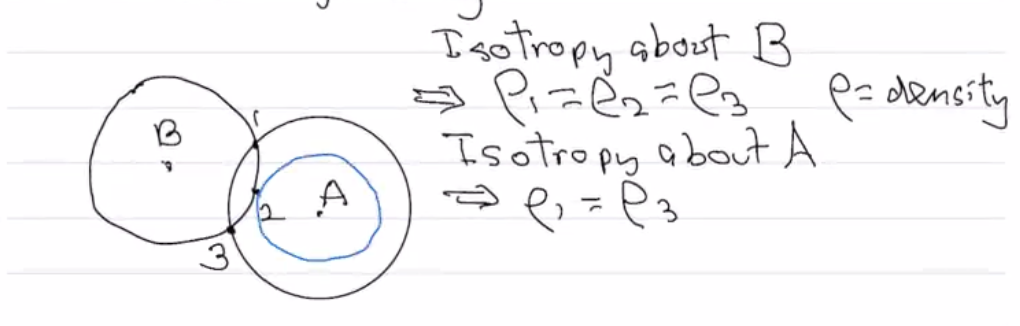
\includegraphics{isotropy.png}
    \caption{Istropy aobut 2 points.}
    \label{fig:isotropy}
\end{figure}

We can consider another example. A homogeneous universe can anisotropic. Consider a homogeneous Universe that is expanding in different directions in a non-uniform way. This leads to different $H_0(x,y,z)$. 

The reason we spend some time on the Cosmological Principle is the \textbf{Friedmann-Robertson-Walker metric}, which we will come to later on.

\subsubsection{Hubble Parameter}

Let's now talk about the \textbf{Hubble parameter}, which is not a constant! It, in fact, changes in time. An empirical linear relationship between the recession speed $v$ and distance $r$ can be seen, called the \textbf{Hubble's Law}:

\begin{equation}
v = H r
\end{equation}

Note that $H_0$ has units of $1/$time. One convention to note is that:

\begin{equation}
H = 100 \underbrace{h}_\text{to hide our ignorance} \frac{\km}{\s \Mpc}
\end{equation}

One useful number to know is $H \approx \frac{h}{10^{10} \yr}$.

Sometimes, when we write $H_0$, we mean the ``present-day'' value ($z = 0$). This is how we will use it now.

\subsubsection{Scale Factor}

We need a language to describe the expansion of the Universe. We will use $a(t)$, which describes the expansion (or contraction) of the Universe. It also relates two different coordinate systems: physical coordinates $\vec{r}$ to comoving coordinates $\vec{x}$. The relation:

\begin{equation}
    \vec{r} = a(t) \vec{x}
\end{equation}

We typically use comoving coordinates in calculations in Cosmology. We can think of $\vec{x}$ as the notches on a stretching ruler. Now consider:

\begin{equation}
    \frac{d}{dt}\vec{r} = \vec{v} = \dot{a} \vec{x} a \vec{\dot{x}}
\end{equation}

\begin{equation}
    \frac{d}{dt}\vec{r} = \vec{v} = \dot{a} \vec{x} a \vec{\dot{x}} = \underbrace{\frac{\dot{a}}{a} \vec{r}}_\text{Hubble} + \underbrace{a \vec{\dot{x}}}_\text{motion relative to expansion (``peculiar velocity'')}
\end{equation}

\begin{equation}
    \boxed{H(t) = \frac{\dot{a}(t)}{a(t)}}
\end{equation}

The name of the game for measuring $H$ is to go far enough that the first term dominates. Otherwise, locally, the second term dominates since peculiar velocities are of order $100$s of $\km/\s$. 

One other convention we need to establish:

\begin{equation}
    a(t_0) = 1 \rightarrow \text{comoving} = \text{today}
\end{equation}

\subsection{The Friedmann Equation; The Equation of State; Radiation, Matter, and Dark Energy}

\subsubsection{The Friedmann Equation}

Below, we will use and derive these, but I am putting the equations at the top for convenience. 

\begin{equation}
    \boxed{\left(\frac{\dot{a}}{a}\right)^2 = \frac{8\pi}{3} G \rho - \frac{kc^2}{a^2}}
\end{equation}

\begin{equation}
    \boxed{\dot{\rho} = -3 \frac{\dot{a}}{a} \left(P + \rho\right)}
\end{equation}

\begin{equation}
    \boxed{\frac{\ddot{a}}{a} = - \frac{4\pi G}{3}\left(\rho +  3P\right)}
\end{equation}

Let's motivate the origin with quasi-Newtonian physics. We can derive it from General Relativity, but that's overkill.

If we assume isotropy, we only need to worry aobu the radial coordinate $r$, not $\theta$ or $\phi$. Homogeneity tells us that $\rho = \text{constant}$ spatially, but \textit{can} depend on time. We will model the Universe as an expanding, homogeneous medium that is adiabatically ($\Delta s =0$) expanding. If it were not adiabatically expanding, we would have heat flow and thus no isotropy. 

With these conditions, let's examine the motion of a thin, expanding, spherical shell of radius $a$. This depends \textbf{only} on the enclosed mass within $a$\footnote{see Birkhoff's Theorem for General Relativity proof}:


\begin{equation}
    M(<a) = \frac{4}{3}\pi a^3 \rho
\end{equation}

Let's consider the energy:


\begin{equation}
    E = \frac12 \dot{a}^2 - \frac{GM}{a}
\end{equation}


\begin{equation}
E = \frac12 \dot{a}^2 - \frac43 \pi G \rho a^2
\end{equation}

Let's re-write $E$ a bit: $k c^2 \equiv -2E$. Note that $k \propto 1/\text{length}^2$. There are three possibilities for $kc^2$:

\begin{itemize}
    \item $>0$, $E<0$, bound
    \item $=0$, $E=0$, critical
    \item $<0$, $E>0$, unbound
\end{itemize}

Let's now evoke the First Law of Thermodynamics ($\Delta S = 0$):

\begin{equation}
   \underbrace{\mathrm{d}U}_\text{internal energy} = -P \mathrm{d}V 
\end{equation}

We now equation the internal energy to the rest-mass energy:

\begin{equation}
    \mathrm{d}\left(\rho c^2 a^3\right) = -P \mathrm{d}\left(a^3\right)
\end{equation}

We will now set $c = 1$ and take a time derivative:

\begin{equation}
    \dot{\rho} a^3 + 3 \rho a^2 \dot{a} = -3P a^2 \dot{a}
\end{equation}

\begin{equation}
    \dot{\rho} -3\frac{\dot{a}}{a}\left(P + \rho\right)
\end{equation}

Using this result and the energy equation from above

\begin{equation}
    \left(\frac{\dot{a}}{a}\right)^2 = \frac{8\pi}{3}G \rho - \frac{k (c)^2}{a^2}
\end{equation}

to get a new equation. If you stare at it hard enough and have divine intervention, take a derivative of the second equation and multiply by $a^2$. Doing so, you get:

\begin{equation}
    2 \dot{a} \ddot{a} = \frac{8\pi}{3}G\frac{d}{dt}(\rho a^2) = \frac{8\pi}{3}Ga^2\left(\dot{\rho} + 2\frac{\dot{a}{a}}\rho\right)
\end{equation}

Simplifying with the other above equation, we get:

\begin{equation}
    2\dot{a}\ddot{a} = -\frac{8\pi}{3}Ga^2 \left(\frac{\dot{a}}{a}\rho + 3\frac{\dot{a}}{a}P\right)
\end{equation}

Simplifying:

\begin{equation}
    \frac{\ddot{a}}{\dot{a}} = -\frac{4\pi}{3}G \left(\rho + 3P\right)
\end{equation}

Note that this is not independent from the other equations; rather it is massaged. Let's compare this to $1$-D Newtonian forces:

\begin{equation}
    \ddot{x} = -\frac{GM}{x^2} = -\frac{4}{3}\pi G \rho x
\end{equation}

\begin{equation}
    \frac{\ddot{x}}{x} = -\frac{4}{3}\pi G \rho 
\end{equation}

Had we done strictly Newtonian physics, we would have never gotten the $+3P$ term. The way to interpret this: we can think of $\rho$ to have an extended meaning: $\rho_{eff} = \rho + 3P$. 

The Grand Summary so far: two equations of motion for $a(t)$: 

\begin{equation}
    \frac{\ddot{a}}{\dot{a}} = -\frac{4\pi}{3}G \left(\rho + 3P\right)
\end{equation}

\begin{equation}
    \dot{\rho}= -3\frac{\dot{a}}{a}\left(P + \rho\right)
\end{equation}

Note this second equation tells us the acceleration! Very importantly, we have a minus sign. If $\rho$ and $P$ are positive, the Universe is \textbf{decelerating}! Conversely, if you have a \textit{bizarre} $P$ and could reverse the parenthetical term, we can have accelerated expansion! 


Right now, we have three unknowns ($P, \rho, a$). How do we get that last piece -- the equation of state ($P \iff \rho$ dependence)?

\subsubsection{Equation of State}

We choose to write:

\begin{equation}
    P = w\rho (c^2)
\end{equation}

We are in units where $c = 1$, but I threw it in for reference. Note -- this means that pressure is the same thing as energy density! Think of the units. 

With that definition of $P$, we can re-write the second boxed equation from above:

\begin{equation}
    \dot{\rho} -3\frac{\dot{a}}{a}\left(1+w\right)\rho
\end{equation}

\begin{equation}
    \frac{\dot{\rho}}{\rho} = -3 (1+w) \frac{\dot{a}}{a} \rightarrow \rho \propto a ^{-3(1+w)}
\end{equation}

\begin{equation}
    \boxed{\rho \propto a^{-3\left(1+w\right)}}
\end{equation}

\textbf{assuming that} $\dot{w} =0$ \textbf{which might not be true}!

\subsubsection{Matter, Radiation, and Dark Energy}

Let's look at a few special cases of the equation of state:

\begin{itemize}
    \item Matter: Non-relativistic, pressure-less particles like cold dark matter. In this case, $w = 0, P = 0 \rightarrow \boxed{\rho \propto a^{-3}}$. This makes sense because it is units of $1/\text{volume}$.
    \item Radiation: Relativistic particles, photons and neutrinos. In this case, $w = 1/3, P = \frac13 \rho \rightarrow \boxed{\rho \propto a^{-4}}$. This makes sense because it is units of $\left(1/\text{volume}\right)\left(1/\text{length}\right) $ where the extra factor is from redshifting energy.
    \item The Cosmological Constant: In this case, $w = -1, P=-\rho \rightarrow \rho = \text{constant}$.
    \item Dark Energy: More general term, where $w < -\frac13$ to make $\ddot{a} >0$.
\end{itemize}

\begin{figure}
    \centering
    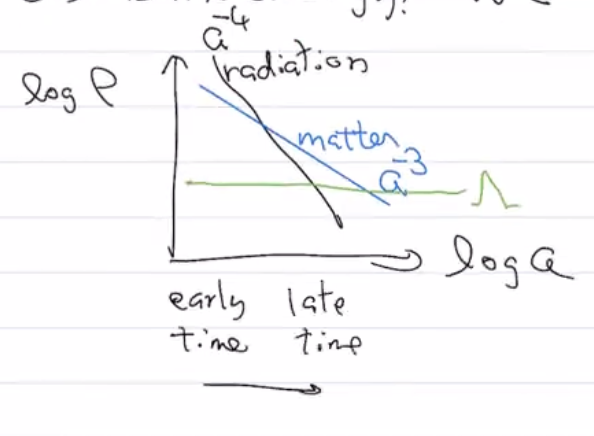
\includegraphics{density.png}
    \caption{Sketch of density over cosmic time. }
    \label{fig:density}
\end{figure}

\subsection{The Density Parameter; Open, flat, closed models; Redshift}

Let's first define $\Omega$ in terms of the \textbf{critical density} $\rho_c$. This is defined to be the density needed to make the Universe flat. Recall the Friedmann Equation:

\begin{equation}
    \left(\frac{\dot a}{a}\right)^2 = \frac{8\pi}{3}G\rho - \frac{k}{a^2}
\end{equation}

First, set $k = 0 \iff E = 0$, then solve for $\rho$:

\be
    \boxed{\rho_c = \frac{3H^2}{8\pi G}}
\ee

This critical density can be interpreted as well as the mean density of a flat Universe ($k=0$). Importantly, $\rho_c$ is a function of $H$, which itself is a function of time. Setting $H = H_0$, we can get Today's value of $\rho_c$:

\be
    \rho_{c,0} = \frac{3H_0^2}{8\pi G} = 2.78 \times 10^{11} h^2 \frac{M_\odot}{\Mpc^3} = 1.88 \times 10^{-29} h^2 \frac{\g}{\cm^3}
\ee

This is about $10^{-5} h^2 m_{proton} \cm^{-3}$. Here are a few other useful numbers to carry around as well:

\be
    \rho_{thumb} \sim 1 \frac{\g}{\cm^3}
\ee

\be
    \rho_{ISM} \sim 1 \frac{m_p}{\cm^3}
\ee

\be
    \rho_{Universe} \sim 1 \rho_c
\ee

Now with these definitions, we have the \textbf{density paramater}:

\be
\Omega(t) \equiv \frac{\rho(t)}{\rho_c(t)} = \frac{8\pi G \rho(t)}{3H^2(t)}
\ee

There are three obvious possibilities:

\begin{itemize}
    \item $\Omega <1 \rightarrow$ Open Universe ($k<0$)
    \item $\Omega = 1\rightarrow$ Flat Universe ($k=0$)
    \item $\Omega >1 \rightarrow$ Closed Universe ($k>0$)
\end{itemize}

There are a few things to note. When we have \textit{mutliple components}, we have:

\be
\Omega(t) = \frac{\sum_{i} \rho_i}{\rho_c}
\ee

where $i$ is often representing radiation, matter, $\Lambda$, baryonic component of matter, dark matter, neutrinos, etc. Another thing we want to stress is that $\rho$, $\rho_c$, $\Omega$ \textbf{all depend on time}. Note that if $\rho > \rho_c$, it will STAY that way. The same goes for $\Omega$, and for other values. For example, these parameters will stay $>, <,$ or $=$ 1. 

\subsubsection{Redshift}

Observationally, we have

\be
1+z \equiv \frac{\lambda_{obs}}{\lambda_{rest}} = \frac{a(t_0)}{a(t)} = \frac{1}{a(t)}
\ee

\be
\boxed{\frac{1}{a(t)} = 1+z}
\ee

\subsection{Time Evolution of Paramaters: Hubble, Density, Scale Factor}

\subsubsection{Hubble Parameter}

Worked out in Problem Set 1, but here is the solution:

\be
H^2(a) = H_0^2 \left(\frac{\Omega_0}{a^{3+3w}} + \frac{1-\Omega_0}{a^2}\right)
\ee

For multiple components (the common ones):

\be
H^2(a) = H_0^2 \left(\frac{\Omega_{0,m}}{a^{3}} + \Omega_{0,\Lambda} + \frac{\Omega_{0,r}}{a^{4}}+ ... + \frac{1-\Omega_{0,m}-\Omega_{0,\Lambda}-\Omega_{0,r}}{a^2}\right)
\ee

\subsubsection{Density Parameter}

First, recall the critical density:

\be
\rho_c = \frac{3 H^2}{8\pi G} \rightarrow H^2 \Omega = \frac{8\pi}{3}G\rho
\ee

We can also look at the Friedmann equation:

\begin{equation}
    \left(\frac{\dot a}{a}\right)^2 = \frac{8\pi}{3}G\rho - \frac{k}{a^2}
\end{equation}

We can replace the first term on the right hand side and set $a=1$:

\be
k = H_0^2 \left(\Omega_0-1\right)
\ee

All of these together, we get:

\be
H^2 = H^2 \Omega - \frac{H_0^2 \left(\Omega_0-1\right)}{a^2}
\ee

Rearrange:

\be
1 - \Omega(a) = \frac{H_0^2}{H^2a^2}\left(1-\Omega_0\right)
\ee

We can use the time evolution of the Hubble Parameter to replace the $H$ terms, leaving:

\be
\boxed{1-\Omega(a) = \frac{1-\Omega_0}{\frac{\Omega_0}{a^{1+3w}} + 1-\Omega_0   }}
\ee

To be more explicit, let's write out the multi-component again:

\be
1 - \Omega(a) = \frac{1 - \Omega_0}{1 - \Omega_0 + \left(\Omega_{m,0}a^{-1} + \Omega_{0,\Lambda}a^{2} + \Omega_{r,0}a^{-2}\right)}
\ee

where $\Omega_0 = \sum_i \Omega_{0,i}$. Note that the above equation essentially FORCES $\Omega(a) \sim 1$. This foreshadows the Flatness Problem.

\subsubsection{Scale Factor (Flat Case)}

This is essentially solving the Friedmann Equation for $a(t)$ for specific models (can, in general, be integrated). The most basic model is the Einstein-de Sitter model: a model that is flat $k = 0 \rightarrow \Omega =1$:

\be
\left(\frac{\dot a}{a}\right)^2 = \frac{8\pi}{3}G\rho
\ee

We have also see that $\rho \propto a^{-3(1+w)}$. Therefore:

\be
\mathrm{d} a a^{\frac32 (1+w)-1} \propto \mathrm{d}t
\ee

\be
\boxed{a(t) \propto t^{\frac{2}{3(1+w)}}}
\ee

Recall for the Einstein-de Sitter model ($k=0, \Omega=0$), we found:

\be
a \propto t^{\frac{2}{3(1+w)}}
\ee

This is very useful since it works for each epoch (matter dominated, radiation dominated, dark energy dominated, etc;, but not in the transitions):

\textbf{Matter Dominated Era} ($w=0, P\approx0$)

\begin{equation}
    \boxed{a_{m}\propto t^{\frac23}}
\end{equation}

\textbf{Radiation Dominated Era} ($w=\frac13, P=\frac13 \rho$)

\begin{equation}
    \boxed{a_{r}\propto t^{\frac12}}
\end{equation}

$\Lambda$ \textbf{Dominated Era} ($w=-1$ (for example), $P=-\rho$)

\begin{equation}
    a_{r}\propto t^{\infty} \rightarrow \text{ Wrong! }
\end{equation}

This breaks down because $H$ is a constant in this case! So here:

\be
    a \propto e^{Ht}
\ee

Isn't this reminiscent of inflation? That's because it is! It wasn't the Cosmological Constant but rather a scalar field called the inflaton.  


\subsubsection{Scale Factor (Open Case)}

Let's consider $k<0$ and $\Omega <1$. Additionally, we assume $\Lambda =0$ and that we are matter-dominated. 

Start with the Friedmann Equation:

\be
\frac{\dot a^2}{a^2} = \frac{8\pi}{3}G\rho - \frac{k}{a^2} > 0 \text{ always}
\ee

Immediately, we see that expansion will never stop! The right hand side is always positive, and therefore $\dot a$ is never equal to $0$. Now, recall the equation for $H(a)$ and the fact that $H = \dot{a}/a$:

\be
\dot{a}^2 = H_0^2 \left(\frac{\Omega_0}{a^{1+3w}} + 1 - \Omega_0\right)
\ee

We now solve for $a(t)$ for this Universe:

\be
\int_0^{a_f} \frac{\mathrm{d}a}{\sqrt{\frac{\Omega_0}{a} + 1 - \Omega_0}} = \int_0^{t_f} H_0 \mathrm{d}t
\ee

The right hand side is easy. The left hand side? Let's start with completing the squares to get rid of the $\frac{1}{a}$, so let's set that up.

\be
\int_0^{a_f} \frac{a \mathrm{d}a}{\left(1-\Omega_0\right)\sqrt{a^2 + \frac{\Omega_0}{1-\Omega_0}a }}
\ee

Now we can actually complete the square in the denominator. Define $2\alpha\equiv \frac{\Omega_0}{1-\Omega_0}$:

\be
\int_0^{a_f} \frac{a\mathrm{d}a}{\sqrt{1-\Omega_0} \sqrt{\left(a + \alpha\right)^2 - \alpha^2}}
\ee

We will now shift variables: $a\prime \rightarrow a + \alpha$:

\be
\int_\alpha^{a_f + \alpha} \frac{\left(a-\alpha\right)\mathrm{d}a}{\sqrt{1-\Omega_0} \sqrt{a^2 - \alpha^2}}
\ee

We can now do trigonometric substitution. Let $a\equiv \alpha \cosh \theta$. This gives $\mathrm{d}a = \alpha \sinh\theta \mathrm{d}\theta$. Lastly, $\sqrt{a^2\alpha^2} = \alpha\sinh\theta$. Properly adjusting limits, we get the expression:

\be
\boxed{a(\theta) = \frac{\Omega_0}{2\left(1-\Omega_0\right)}\left(\cosh\theta-1\right)}
\ee

\be
\int_{0}^{\theta_f} \frac{\alpha^2\left(\cosh\theta-1\right)\sinh\theta}{\sqrt{1-\Omega_0} \alpha \sinh\theta} \mathrm{d}\theta
\ee

\be
\frac{\alpha}{\sqrt{1-\Omega_0}}\left(\sinh\theta - \theta\right)\rvert_0^{\theta_f}
\ee

\be
H_0 t_f = \frac{\Omega_0}{2\left(1-\Omega_0\right)^{3/2}} \left(\sinh\theta_f -\theta_f\right)
\ee

This gives:

\be
\boxed{t(\theta) = \frac{\Omega_0}{2H_0\left(1-\Omega_0\right)^{3/2}}\left(\sinh\theta - \theta\right)}
\ee

We can then use $\theta$ as some parameter, trace out $a$ and $t$, and then find $a(t)$!

\subsubsection{Scale Factor (Closed Case)}

You can repeat the derivation above for the matter-dominated, closed case of $k >0$, $\Omega > 1$. Here, there \textit{will} be a maximum of $a$ and the dynamics are different $\theta \rightarrow i \theta$):

\be
\boxed{t(\theta) = \frac{\Omega_0}{2H_0\left(\Omega_0-1\right)^{3/2}}\left(\theta-\sin\theta\right)}
\ee

\be
\boxed{a(\theta) = \frac{\Omega_0}{2\left(\Omega_0-1\right)}\left(1-\cos\theta\right)}
\ee

\subsubsection{Deceleration Parameter}

Let's define this -- it was used historically since we now know the Universe is \textit{accelerating}. This is a dimensionless parameter:

\be
q \equiv -\frac{\ddot{a}a}{\dot{a}^2} \rightarrow q = - \frac{1}{H^2} \frac{\ddot{a}}{a}
\ee

Recall one of the other results we had this semester:

\be
\frac{\ddot{a}}{a} = -\frac{4\pi}{3}G\left(\rho+3P\right)
\ee

and

\be
\rho_c = \frac{3H^2}{8\pi G} \rightarrow H^2 \Omega = \frac{8\pi}{3}G\rho
\ee

Putting this together with $q$:

\be
\frac{\ddot{a}}{a} = -\frac{4\pi}{3}G\rho \left(1+3w\right) = -\frac{H^2 \Omega}{2}\left(1+3w\right)
\ee

This makes:

\be
q = \frac{\Omega}{2}\left(1+3w\right)
\ee

For multiple components:

\be
\boxed{q = \sum_i \frac{\Omega_i}{2}\left(1+3w_i\right)}
\ee

\be
q = \frac{\Omega_m}{2} + \underbrace{\frac{1+3w}{2}\Omega_w}_\text{Dark Energy} + \Omega_r + ...
\ee

For a matter-dominated Universe and $\Omega_\Lambda \neq 0$:

\be
\boxed{q = \frac{\Omega_m}{2} - \Omega_\Lambda}
\ee

\textbf{The minus sign there is enormously important!}

One thing to note: supernovae are sensitive to $q$, whereas CMB measurements are sensitive to the addition of $\Omega_m$ and $\Omega_\Lambda$, so in some sense, these are orthogonal instead of parallel. 

\subsection{Robertson-Walker Metric}

This is where you would start in General Relativity. 

Let's set up the background. Recall Lorentz transformations in Special Relativity. There are two inertial observers, $(x,y,z,t)$ and $(x',y',z',t')$ with relative velocity $\vec{v}=v\hat{x}$:

\be
x' = \gamma(x-vt)
\ee

\be
y' = y
\ee

\be
z' = z
\ee

\be
t' = \gamma\left(t-\frac{vx}{c^2}\right)
\ee

We also talked about the Lorentz invariant interval:

\be
\mathrm{d}s^2 = c^2 \mathrm{d}t^2 - \left(\mathrm{d}x^2 + \mathrm{d}y^2 + \mathrm{d}z^2\right) = \mathrm{d}s'^2
\ee

Recall that the propagation of light follows the ``null geodesic'': $\mathrm{d}s^2 = 0$:

\be
\mathrm{d}r = c\mathrm{d}t
\ee

We will quote the RW Metric here, and explore it next time. In short, Robertson and Walker showed that, for a \textbf{homogeneous and isotropic space, the most general metric is} (see Weinberg for a full proof):

\be
\mathrm{d}s^2 = c^2 \mathrm{d}t^2 - a^2\left(t\right) \left[\frac{\mathrm{d}r^2}{1-kr^2} + r^2 \left(\mathrm{d}\theta^2 + \sin^2\theta \mathrm{d}\phi^2\right) \right]
\ee

We are defining the coordinates as:

\begin{figure}
    \centering
    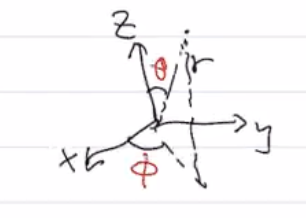
\includegraphics[width=0.75\textwidth]{coordinates.png}
    \caption{Spherical coordinate convention. }
    \label{fig:coords}
\end{figure}

An immediate and obvious consequence is when $k=0$, where we recover the Minkowski metric for flat space. 
Let's consider the more interesting cases of open ($k<0$) and closed ($k>0$). Immediately, we have a coordinate singularity at $r = \frac{1}{\sqrt{k}}$. Recall that $k = \frac{H_0^2}{c^2} \left(\Omega_0-1\right)$. We can thus define the \textbf{radius of curvature}:

\be
R_0 \equiv \frac{1}{\sqrt{k}} = \frac{c}{H_0} \left(\frac{1}{\sqrt{\Omega_0-1}}\right)
\ee

Let's step back a second and look at the form of the FRW metric with some analogies:

$$\begin{matrix} 
\text{3-sphere (in 4D)} & \text{2-sphere (in 3D)}\\
(x,y,z,w)\iff (R,\alpha,\beta,\gamma)&(x,y,z)\iff(R,\theta,\phi)\\
w=R\cos\alpha&z=R\cos\theta\\
z=R\sin\alpha\cos\beta&y=R\sin\theta\cos\phi\\
y=R\sin\alpha\sin\beta\cos\gamma&x=R\sin\theta\sin\phi\\
x=R\sin\alpha\sin\beta\sin\gamma& \\
x^2+y^2+z^2+w^2=R^2&x^2+y^2+z^2=R^2\\
\end{matrix}$$

Look at a line element of the 2-sphere embedded in 3D:

\be
\mathrm{d}\ell^2 = R^2\left(\mathrm{d}\theta^2 + \sin^2\theta \mathrm{d}\phi^2\right)
\ee

We will change variables to $u = \sin\theta \rightarrow \mathrm{d}u = \cos\theta \mathrm{d}\theta = \sqrt{1-u^2}\mathrm{d}\theta$. This makes the line element:

\be
\mathrm{d}\ell^2 = R^2 \left(\frac{\mathrm{d}u^2}{1-u^2} + u^2 \mathrm{d}\phi^2\right)
\ee

Look at that! We're not quite there, but we have a similar form to the metric we want! 

And the line element of the 3-sphere embedded in 4D:

\be
\mathrm{d}\ell^2 = R^2\left(\mathrm{d}\alpha^2 + \sin^2\alpha \mathrm{d}\Omega^2\right)
\ee

where 

\be
\mathrm{d}\Omega^2 \equiv \mathrm{d}\beta^2 + \sin^2\beta \mathrm{d}\gamma^2
\ee

Again, we can change variables, $u \equiv \sin\alpha \rightarrow \mathrm{d}u = \sqrt{1-u^2}\mathrm{d}\alpha$:

\be
\mathrm{d}\ell^2  =R^2 \left[\frac{\mathrm{d}u^2}{1-u^2} + u^2 \mathrm{d}\Omega^2 \right]
\ee

Again, where

\be
\mathrm{d}\Omega^2 \equiv \mathrm{d}\beta^2 + \sin^2\beta \mathrm{d}\gamma^2
\ee

Compared to the Friedmann-Robertson-Walker metric, these are identical! 

\be
\frw
\ee

Thus, for a $3$-sphere in 4-dimensions, we recover the FRW metric dependence in a hand-wavy way. 

For the open model ($k<0$), we don't have coordinate singularities. Instead of a spherical analogy, we use a saddle as an analogy (or, more tasty, Pringles!). This case has infinite volume and is called Lobachevsky space. Here, we let $u \equiv \sinh\theta$ which you can see will receover the proper FRW dependence. 

There is an alternative form of the metric, too, we should know. We will see this in Problem Set 2. It is written as:

\be
\mathrm{d}s^2 = c^2 \mathrm{d}t^2 - a^2\left(t\right) \left[\mathrm{d}\chi^2 + \mathcal{S}^2 \left(\mathrm{d}\theta^2 + \sin^2\theta \mathrm{d}\phi^2\right)\right]
\ee

\subsection{Basic Kinematic Properties of the Smooth Universe}

Here, we have in mind:

\begin{itemize}
    \item Comoving radial distance vs. Redshift
    \item Time vs. Redshift
    \item Age of the Universe
    \item Other useful quantities
\end{itemize}

\subsubsection{Comoving, Radial Distance vs. Redshift (``The Hubble Diagram'')}

By the comoving radial distance, we mean the $r$ in the RW metric. 

First, we know that photons follow $\mathrm{d}s^2 = 0$, so let's take a radial path from the observer ($\mathrm{d}\theta = \mathrm{d}\phi = 0$. Now we have:

\be
0 = c^2 \mathrm{d}t^2 - \frac{a^2 \mathrm{d}r^2}{1-kr^2}
\ee

\be
\int_{0}^{r_1} \frac{\mathrm{d}r}{\sqrt{1-kr^2}} = c\int_{t_1}^{t_0} \frac{\mathrm{d}t}{a(t)}
\ee

where $t_0$ is the age of the Universe. Evaluating these integrals, starting with the flat, static Universe ($k=0, a=1$):

\be
\mathrm{d}r = c \mathrm{d}t \rightarrow r = ct
\ee

What about other cases? First, let's replace $\mathrm{d}t$ by $\mathrm{d}z$ using $H = \frac{1}{a}\frac{\mathrm{d}a}{\mathrm{d}t}$ and $a = (1+z)^{-1}$:

\be
H =-\frac{1}{1+z} \frac{\mathrm{d}z}{\mathrm{d}t}
\ee

Also recall:

\be
H\left(z\right) = H_0 
\sqrt{\Omega_0 \left(1+z\right)^{3+3w} + \left(1-\Omega_0\right)\left(1+z\right)^2}
\ee

Thus:

\be
\mathrm{d}t = - \frac{\mathrm{d}z}{H(1+z)} = -\frac{\mathrm{d}z}{H_0\left(1+z\right)\sqrt{\text{stuff}}}
\ee

Going back to our integral expression:

\be
\text{RHS} = \int_{t_1}^{t_0} \frac{c\mathrm{d}t}{a(t)} = \frac{c}{H_0} \int_{0}^{z_1} \frac{\mathrm{d}z}{\sqrt{\text{stuff}}}
\ee

We will look at two cases of the above.

\begin{itemize}
    \item Einstein-de Sitter Model $k = 0, \Omega_0 = \Omega_{0,m} = 1$. No other components. 
    \item  Arbitrary $\Omega_{m,0}$ and $\Omega_{m,\Lambda}$ with negligible radiation. 
\end{itemize}

\noindent\textbf{Einstein-de Sitter}

\begin{equation}
\text{RHS} = \frac{c}{H_0}\int_0^{z_1} \frac{\mathrm{d}z}{(1+z)^{3/2}} = \frac{2c}{H_0}\left[1-(1+z_1)^{-1/2}\right]
\end{equation}

\begin{equation}
\text{LHS} = \int_0^{r_1} \mathrm{d}r = r
\end{equation}

Thus, we have the comoving radial distance for the Einstein-de Sitter Universe:

\be
\boxed{r = \frac{2c}{H_0}\left(1-\left(1+z\right)^{-1/2}\right]}
\ee

Let's examine a few limits. As $z\to\infty$, $r\to\frac{2c}{H_0} \approx 6 h^{-1} \Gpc$. When $z\ll1$, $r\approx \frac{cz}{H_0}$. Note that this is just Hubble's Law! Since, for small $z$, $v \approx cz$. \\

\noindent\textbf{Arbitrary Case}

We will show this in PS2, but in this case:

\be
\boxed{r = |k|^{-1/2} \operatorname{sinn}\{\frac{c}{H_0}|k|^{1/2} \int_0^{z} \frac{\mathrm{d}z^\prime}{\sqrt{\Omega_{0,m}\left(1+z^\prime\right)^3 + \Omega_{0,\Lambda} + \left(1-\Omega_{0,m}-\Omega_{0,\Lambda}\right)\left(1+z^\prime\right)^2}} \}}
\ee

where 

\be
\boxed{\text{sinn} = 
\begin{cases}
\sin \text{ when } k > 0 \\
\text{absent when } k = 0 \\
\sinh \text{ when } k < 0 
\end{cases}
}
\ee

For $z\ll1$, all three cases of $k$:

\be
\boxed{r = \underbrace{\frac{c}{H_0}(z}_\text{Hubble's Law}-\frac{1}{2}\left[1+q_0\right]z^2) + \mathcal{O}(z^3)}
\ee

where 

\be
q_0 = \frac{\Omega_{0,m}}{2} - \Omega_{0,\Lambda} + \Omega_{0,r}
\ee

This is an enormously important equation, historically. Again, here we see that the Supernova experiments depend on $q_0$, thus the \textbf{difference} between $\Omega_{0,m}$ and $\Omega_{0,\Lambda}$, allowing good constraints. 

\subsubsection{A Note on Various Distances}

There are two other commonly used cosmological ``distances'':

\begin{itemize}
    \item Luminosity distance
    \item Angular diameter distance
\end{itemize}

\noindent\textbf{Luminosity Distance} $D_L$

This is based on standard candles. This is defined to be:

\be
D_L \equiv \sqrt{\frac{L_\text{emit}}{4\pi S_\text{obs}}}
\ee

where the variables are emitted luminosity and observed flux. There are two factors for $1+z$ we have to look out for. For luminosity, we have energy per time. Energy is diluted by $1+z$ and time is dilated by $1+z$, so:

\be
D_L = \left(1+z\right) r_\text{comoving}
\ee

\noindent\textbf{Angular Diameter Distance} $D_A$

This is based on standard rulers. This is defined to be:

\be
D_A \equiv \frac{\ell_\text{physical}}{\underbrace{\theta}_\text{angular size}}
\ee

We can change this to comoving coordinates easily:

\be
D_A = \frac{r_\text{comoving}}{\left(1+z\right)}
\ee

\subsubsection{Time vs. Redshift}

All we need here is $\mathrm{d}t$ vs. $\mathrm{d}z$, integrate, and we are okay. So how do we do that?

We actually did this earlier when we were deriving $H(a)$. Recall:

\be
\mathrm{d}t = -\frac{1}{H_0} \frac{\mathrm{d}z}{\left(1+z\right) \sqrt{\Omega_0 \left(1+z\right)^{3+3w} + (1-\Omega_0)\left(1+z\right)^2}}
\ee

Let's ask a few questions -- what's the time since the Big Bang at redshift $z$?

\be
t = \frac{1}{H_0}\int_{z}^{\infty} \frac{\mathrm{d}z^\prime}{\left(1+z^\prime\right)\sqrt{\Omega_0 \left(1+z\right)^{3+3w} + (1-\Omega_0)\left(1+z\right)^2}}
\ee

A related question -- what's the age of the Universe today? All we do is set $z = 0$ above! 

\be
t_0 = \frac{1}{H_0}\int_{0}^{\infty} \frac{\mathrm{d}z^\prime}{\left(1+z^\prime\right)\sqrt{\Omega_0 \left(1+z\right)^{3+3w} + (1-\Omega_0)\left(1+z\right)^2}}
\ee

Again, as always, let's look at a few special cases, starting with EdS:

\noindent\textbf{Einstein de Sitter}
\be
t_0 = \frac{1}{H_0} \int_)^\infty \frac{\mathrm{d}z}{(1+z)^{5/2}} = -\frac{2}{3H_0} \left(1+z\right)^{-3/2}\rvert_{0}^{\infty} =\frac{2}{3H_0}
\ee

A different way to derive this -- recall that $a(t) \propto \left(\frac{t}{t_0}\right)^{2/3}$. Thus, $H = \frac{\dot{a}}{a} = \frac23 \frac{1}{t}$. We can set this to today: $t_0 = \frac{2}{3H_0}$. Remind yourself that $H_0^{-1} = 10^{10} h^{-1} \yr$. This gives:

\be
t_0 \approx 6.7 h^{-1} \Gyr
\ee

Now, another case, where $k=0$ but allow for non-zero $\Omega_{0,\Lambda}$ (but $\Omega_m + \Omega_\Lambda = 1$. We can show this, but we won't, that:\\

\be
t_0 = \frac{2}{3H_0}\frac{1}{\sqrt{\Omega_{0,\Lambda}}}\ln \left(\frac{1 + \sqrt{\Omega_{0,\Lambda}}}{\sqrt{\Omega_{0,m}}}\right) \approx \frac{2}{3H_0}\Omega_{0,m}^{-0.3}
\ee


\noindent\textbf{Open Case}

Here, we will consider $k<0$, $\Omega_0<1$ and matter only. We looked at this extensively when we did parametric solutions:

\be
t(\theta) = \frac{\Omega_0}{2H_0\left(1-\Omega_0\right)^{3/2}}\left(\sinh\theta - \theta\right)
\ee

\be
a(\theta) = \frac{\Omega_0}{2\left(1-\Omega_0\right)}\left(\cosh\theta - 1\right)
\ee

Today, we have $a(\theta_0) = 1 \rightarrow \cosh\theta_0 = \frac{2-\Omega_0}{\Omega_0}$. After a little bit of algebra, we find:

\be
\sinh\theta_0 = \frac{2}{\Omega_0}\sqrt{1-\Omega_0}
\ee

\be
t_0 = \frac{1}{H_0} \left[(1-\Omega_0)^{-1} - \frac12 \Omega_0 \left(1-\Omega_0\right)^{-3/2}\cosh^{-1}\left(\frac{2-\Omega_0}{\Omega_0}\right) \right]
\ee

We can show that:

\be
t_{0,\text{open}} > \frac{2}{3H_0} (t_0 \text{ for flat})
\ee

Additionally, if we take $\Omega_0 \to 0$ (a \textbf{Milne} Universe), then $t_0 \to \frac{1}{H_0}$.\\

\noindent\textbf{Closed Case}

This is when $\Omega_0 > 1$, with matter only, and $k>0$. Correspondingly, we get:

\be
t_0 = \frac{1}{H_0} \left[(1-\Omega_0)^{-1} + \frac12 \Omega_0 \left(\Omega_0 - 1\right)^{-3/2}\cos^{-1}\left(\frac{2-\Omega_0}{\Omega_0}\right) \right]
\ee

We can show that:

\be
t_{0,\text{closed}} < \frac{2}{3H_0} (t_0 \text{ for flat})
\ee

Note that there is a nice identity: $\cosh^{-1}(x) = \ln\left(x + (x^2-1)^{1/2}\right)$. 


\section{The Bright Universe}

We have discussed the smooth, Friedmann-Roberston-Walker Universe. What about fluctuations in density? Let's fill the Universe in, starting with the bright stuff (baryons). This climaxes with the Big Bang, and the prediction of mass ratios of the elements H, He, D, and $^7$Li (with very minor tension). The thermodynamics that we learn here differs in that we have an expanding background with different particles with different statistics. 

We must then compare the expansion rate (Hubble Rate) to the particle interactions that keep things in equilibrium. 

\subsection{The Planck Mass: The Ugliest Numbers in Physics}

This might just look like unit conversion tricks in various branches physics:

\begin{itemize}
    \item High Energy Physics
    \begin{itemize}
        \item Energy $\sim \frac{1}{\text{length}}$, with $\hbar c \approx 200 \text{ fermi-MeV}$ where $1 \text{fermi} = 10^{-13} \cm$ and $\hbar \equiv \frac{h}{2\pi}$. The convention is to instead say $\hbar c =1$. Nominally, this says:
        
        $$
        1 \text{ MeV} \approx \frac{1}{200} \text{ fermi}
        $$
        
        \item Energy $\sim$ mass, so $c = 1$. Thus, 
        
        $$
        1 \text{ GeV} \approx m_p \approx 1.67\times 10^{-24} \g
        $$
    \end{itemize}
    
    \item Condensed Matter Physics 
    \begin{itemize}
        \item Energy $\sim$ Temperature, and the way we do this is setting $k_B T_{\text{room, }300\text{ K}} = \frac{1}{40} \text{ eV}$. An easy example is the CMB, which has a temperature of around $3 \text{ K}$. Immediately, the characteristic photon energy is thus $\frac{1}{4000} \text{ eV}$, or around $2.5 \times 10^{-4} \text{ eV}$. As a side note, if we want to say if something is ``relativistic,'' we have to compare the particle's rest mass to the characteristic photon energy at a given temperature. 
        
        $$
        k_B T_{\text{room, }300\text{ K}} = \frac{1}{40} \text{ eV}
        $$
    \end{itemize}
    
    \item Astrophysics
    \begin{itemize}
        \item Here, we look to the Schwarzschild radius of the Sun:
        
        $$
        R_\text{Sch} = \frac{2GM}{c^2}
        $$
        
        Pinning this to the sun, we get $R_\text{Sch} \approx 3 \text{ km}$. 
    \end{itemize}
\end{itemize}

So how does this relate to the Planck Mass? This is scale at which gravity and quantum mechanics are comparable in strength. We also call this the ``unifying scale'' of gravity and quantum mechanics. For gravity, this scale is $R_\text{Sch}$ and for QM, this is $\lambda_c = \frac{hc}{mc^2} = \frac{2\pi \hbar c}{mc^2}$. When $R\sim \lambda$ and $m_\text{pl}$:

$$
\frac{G m_\text{pl}}{c^2} = \frac{\hbar c}{m_\text{pl}c^2} \rightarrow \boxed{m_\text{pl} = \sqrt{\frac{\hbar c}{G}} \approx 1.22\times 10^{19} \text{ GeV} }
$$

Schematically, we have:

\begin{figure}
    \centering
    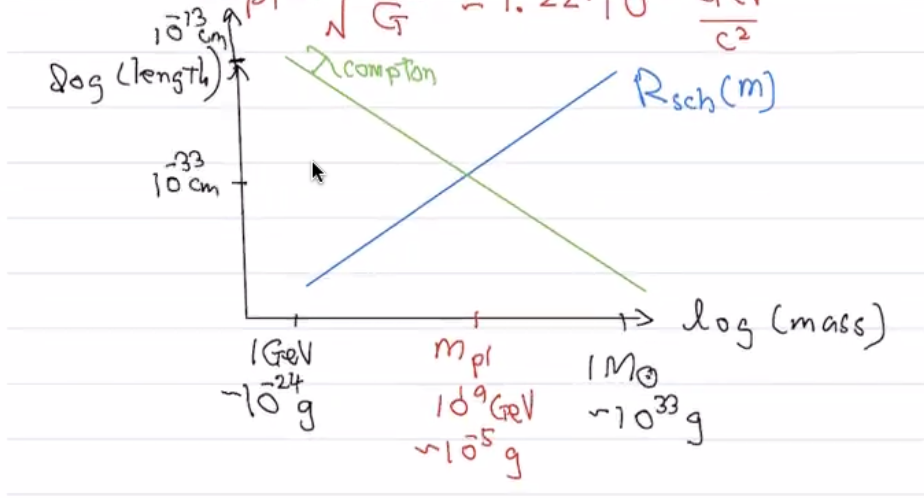
\includegraphics{scales.png}
    \caption{Length and mass scales, with the Planck mass being the intersection. }
    \label{fig:scales}
\end{figure}

A very natural scale for $\Lambda$ would be the Planck mass, right? Let's check that, looking at the Energy density in $\Lambda$ to order of magnitude:

\be
\Omega_\Lambda = 0.7 \approx 1 \rightarrow \rho_\Lambda \sim \rho_{c} \sim 1 \times 10^{-5} h^2 \frac{\unit{GeV}}{\unit{cm}^3}
\ee

Re-writing this with our conventions above (that $200 \unit{MeV} \approx \unit{fm}^{-1} \sim 10^{13} \cm^{-1}$. 

\be
\frac{1}{\cm^3} \sim \left(0.2 \unit{GeV}\right)^3\times 10^{-39} \sim 10^{-41} \unit{GeV}
\ee

Thus

\be
\boxed{\rho_\Lambda \sim 10^{-46} \unit{GeV}^4} 
\ee

Here comes the comparsion that should shock you. What's the natural scale, again? The Planck Scale! So how does $\rho_\Lambda$ compare with $m_\text{pl}^4$. 

\be
\boxed{m_\text{pl}^4 \sim 10^{76} \unit{GeV}^4}
\ee

Notice!

\be
\frac{\rho_\Lambda}{m_{pl}^4} \sim 10^{-122}
\ee

Why the heck is that so small? It's so ugly, unnatural, and not $\mathcal{O}(1)$.


\subsection{Thermodynamics in an Expanding Universe}


Here, we have lots of review of thermodynamics but applied to a non-static, fluid background. The conditions in the Early Universe (the first three minutes, or so). We had extremely high temperature, high pressure, and high density (either energy density $\rho$ or number density $n$). To a good approximation, though not always true, we have thermal equilibrium. Additionally, we can treat all these particles as if they are ideal gases -- gases where interactions are negligible. 

In phase space, we can have a phase space volume: $\mathrm{d}^3x \mathrm{d}^3 p$ which has units of $h_\text{planck}^3$. We use the term \textbf{phase space distribution function} $f(\vec{x},\vec{p},t)$, by the way. We thus have that:

\be
\text{Particle No.: } \mathrm{d}N = f(\vec{x},\vec{p},t) \frac{\mathrm{d}^3x \mathrm{ d}^3p}{h^3} g
\ee

When thermodynamics breaks down, we always can return to the evolution of $f$ directly, which is goverened by the \textbf{Boltzmann equation}. On a good day, we don't have to solve the 6-dimensional Boltzmann equation and can return to fluid dynamics instead. On a bad day, we have to return to our distribution function analysis. 

Now, recall from statistical mechanics: the equilibrium occupation number of a state of energy $\epsilon(p)$:

\be
f = \frac{1}{e^\frac{\epsilon-\mu}{kT} \pm 1}
\ee

where $+$ is for fermions  and $-$ is for bosons. Note as well that $\mu$ is the chemical potential:

\be
\mathrm{d}U =T \mathrm{d}S - P\mathrm{d}V + \mu \mathrm{d}N
\ee

The physical meaning of $\mu$ is thus the change in internal energy due to change in particle number! For a thermal radiation background, we have $\mu = 0$. This will be the case for most astrophysical contexts. 

The most obvious consequence of the above Boltzmann statistics is that the temperature evolves in time, but thermal equilibrium gives us spatial homogeneity. We need to know the first order perturbations to $f$ if we want to consider the non-linear Universe (the CMB!). 

Here are a few macroscopic, useful quantities:

\begin{itemize}
    \item Number density (where $\epsilon(p) = \sqrt{m^2 c^4 + p^2 c^2}$: 
    \be
    n = \frac{g}{h^3} \int_{0}^{\infty} \frac{4\pi p^2 }{e^\frac{\epsilon(p)}{kT} \pm 1}\mathrm{d}p
    \ee
    
    \item Energy density $u$:
    
    \be
    u = \rho = \frac{g}{h^3} \int_{0}^{\infty} \epsilon(p) \frac{4\pi p^2 }{e^\frac{\epsilon(p)}{kT} \pm 1}\mathrm{d}p
    \ee
    
    \item Entropy density $s$:
    \be
    s \equiv \frac{S}{V} = \frac{1}{V}\frac{1}{T} \left(U + PV - \mu N\right)
    \ee
    
    when $\mu = 0$:
    
    \be
    s = \frac{u+P}{T} 
    \ee
\end{itemize}


\noindent\textbf{Two limits:}
We will see familiar expressions when we take some limits. Starting with the \textbf{ultrarelativistic limit} $kT \gg mc^2$.\footnote{Note, again, that $T$ changes in time and therefore particles change from ultrarelativistic to non-relativistic throughout the evolution of the Universe. } Here, the particles are effectively massless and $\epsilon \rightarrow pc$. Computing these integrals:

\begin{itemize}
    \item Number density:
    \be
    n = \frac{g}{h^3}\int_0^\infty \frac{4\pi p^2}{e^{\frac{pc}{kT}} -1} \mathrm{d}p = \frac{4\pi g}{(2\pi)^3} \left(\frac{kT}{\hbar c}\right)^3 \int_0^\infty \frac{y^2}{e^{y} -1} \mathrm{d}y  
    \ee
    
    \item Energy density
    
    \be
    u = \frac{4\pi g}{(2\pi)^3}\left(\frac{k^4T^4}{\hbar^3 c^3}\right) \int_0^\infty \frac{y^3 \mathrm{d}y}{e^y \pm 1}
    \ee
    
    \begin{itemize}
        \item Bosons:
        
        \be
        n = \frac{1}{\Gamma(n)}\int_0^\infty \frac{y^{n-1} \mathrm{d}y}{e^y - 1}
        \ee
        
        We need two results:
        
        \be
        \int_0^\infty \frac{y^{2} \mathrm{d}y}{e^y - 1} = \Gamma(3) \zeta(3)
        \ee
        
        \be
        \int_0^\infty \frac{y^{2} \mathrm{d}y}{e^y - 1} = \Gamma(4) \zeta(4) = \frac{\pi^4}{15}
        \ee
        
        Thus:
        
        \be
        \boxed{n_\text{bosons} = \frac{g}{\pi^2} \zeta(3) \left(\frac{kT}{\hbar c}\right)^3}
        \ee
        \be
        \boxed{u_\text{bosons} = \frac{\pi^2}{30} g \left(\frac{(kT)^4}{(\hbar c)^3}\right)}
        \ee
        
        For photons, this is blackbody radiation since $g=2$ for two polarization states. This also gives us an energy flux of 
        
        \be
        \boxed{F = \frac14 uc = \frac{\pi^2}{60}\frac{k^4}{(\hbar c)^3} T^4 = \sigma T^4}
        \ee
        
        where we introduce $\sigma = \frac{\pi^2 k^4}{60 (\hbar c)^3} = 5.67\times 10^{-8} \frac{\unit{W}}{\unit{m}^2\unit{K}^4}$. An obvious next question -- what's the photon pressure (from equation of state)?
        
        \be
        P = \frac13 u
        \ee
        
        And lastly, the entropy density:
        
        \be
        s = \frac{u+P}{T} = \frac43 \frac{U}{T}
        \ee
        
        One thing that is important to note -- recall that $\rho \propto a^{-4}$ for radiation. Since $u\propto T^4$, $\boxed{T\propto a^{-1}}$ assuming fixed $g$. \textbf{As the Universe cools, the effective} g \textbf{changes}.
        
        \item Fermions:
        
        We can use one trick to make this easy! There's an identity that:
        
        \be
        \frac{1}{e^y + 1} = \frac{1}{e^y - 1} - \frac{2}{e^{2y}-1}
        \ee
        
        where $y = \frac{pc}{kT} \rightarrow 2y = \frac{pc}{k\frac{T}{2}}$.
        
        \be
        n_\text{fermions}(T) = \left[n_B(T) - 2n_B\left(\frac{T}{2}\right) \right]\frac{g_\text{fermions}}{g_\text{bosons}}
        \ee
        
        \be
        n_\text{fermions}(T) = \left[1-2\left(\frac12\right)^3\right] n_B(T) \frac{g_\text{fermions}}{g_\text{bosons}}
        \ee
        
        \be
        \boxed{n_\text{fermions}(T) = \frac{g_\text{fermions}}{g_\text{bosons}} \frac34 n_\text{bosons}(T) }
        \ee
        
        And thus the same thing for the energy density:
        
        \be
        u_\text{fermions}\left(T\right) = \left[u_b(T) - 2u_B\left(T/2\right)\right]\frac{g_f}{g_b}
        \ee
        
        \be
        \boxed{u_\text{fermions}\left(T\right) = \frac{g_\text{fermions}}{g_\text{bosons}} \frac78 u_B\left(T\right)}
        \ee
        
        And similarly, for energy density:
        
        \be
        \boxed{s_\text{fermions}\left(T\right) = \frac{g_\text{fermions}}{g_\text{bosons}} \frac78 s_B\left(T\right)}
        \ee
        
        
    \end{itemize}
    
    For convenience, we can define an effective degeneracy:
    
    \be
    \boxed{g^\star = \sum_\text{boson types} g_i + \frac78 \sum_\text{fermion types} g_i}
    \ee
    
    And thus:
    
    \be
    \boxed{u_\text{Tot} \propto g^\star T^4}
    \ee
    
    
\end{itemize}

\noindent\textbf{Non-relativistic limit:}

This is the case when $kT \ll mc^2$. In this limit, $\epsilon = \sqrt{m^2c^4 + p^2 c^2} \rightarrow mc^2 \left(1+\frac{1}{2}\frac{p^2}{m^2c^2} + ...\right) \gg kT$. Our Fermi-Dirac or Bose-Einstein distribution thus become the same since the $\pm 1$ becomes irrelevant! We drop that in the distribution function for $f$, and thus:

\be
f \sim e^{-\epsilon/kT} \approx e^{-\frac{mc^2}{kT}}\underbrace{e^{-\frac{p^2}{2mkT}}}_{e^{-mv^2/2kT}}...
\ee

Look at that! The second term is a 
Maxwellian distribution! This makes sense -- if we talk about the distribution of stars in a cluster, we don't care if they are bosons!

What about number density? 

\be
n \approx \frac{g}{h^3} \int_0^\infty \mathrm{d} p 4\pi p^2 e^{-\frac{p^2}{2mkT}}
\ee

\be
n \approx \frac{4\pi g}{h^3} \left(2mkT\right)^{3/2} e^{-\frac{mc^2}{kT}} \underbrace{\int_0^\infty \dd{y} y^2 e^{-y^2}}_{\pi^{1/2}/2}
\ee

\be
\boxed{n = \frac{g}{\hbar^3} \left(\frac{mkT}{2\pi}\right)^{3/2} e^{-\frac{\left(mc^2 - \mu\right)}{kT}}}
\ee

where $\mu$ is the chemical potential, sometimes non-zero. The key feature here is that $n$ is exponentially suppressed at $kT \ll mc^2$. For example, at $T \ll 1 \unit{GeV}$ and in thermal equilibrium, neutrons and protons are non-relativistic:

\be
\frac{n_n}{n_p} \approx e^{-\frac{\left(m_n - m_p\right)c^2}{kT}} \approx e^{-\frac{1.293 \unit{MeV}}{kT}}
\ee

Note that neutrons are a bit heavier, and therefore a small under abundant! Also, as temperature drops, so does the ratio $n_n$ to $n_p$. What matters here is at what value is this ratio frozen? This will give us the hydrogen to helium mass ratio! 

\subsection{Thermal History of the Universe: The Longest Three Minutes of Our Lives}

Let's first agree to some rules or questions to ask:

\begin{itemize}
    \item Rule 1: Thermal equilibrium (TE) vs. Decoupling or ``Freeze-Out''\footnote{Decoupling from photons! We might say something like "the photons and electrons froze out at..."}: Need to compare relevant interaction rate $\Gamma$ with Hubble expansion rate $H$ 
    \begin{itemize}
        \item $\Gamma \gg H \rightarrow$ many interactions per Hubble time, and thus can keep equilibrium. 
        \item $\Gamma \ll H \rightarrow$ interactions are negligible, and particles are decoupled
        \item \textbf{Example}: Weak interactions (neutrinos) which freeze-out first since they are so weak:
        \be
        \sigma_\text{weak} \sim G_\text{Fermi}^2 T^2 \sim 10^{-43} \left(\frac{kT}{1 \unit{MeV}}\right)^2 \cm^2
        \ee
        \be
        \sigma_\text{Thomson} \sim 10^{-24} \cm^2 \text{ for reference}
        \ee
        \begin{itemize}
            \item This gives us an interaction rate dependent on $T$:
            \be
            \Gamma_\text{weak} \sim n \sigma_\text{weak} v \propto G_F^2 T^5
            \ee
            \item And we compare this to the Hubble rate:
            \be
            H = \sqrt{\frac{8\pi}{3}G \rho} \propto \sqrt{G g^\star} T^2 \text{ for radiation dom. era}
            \ee
            \item So when are neutrinos in equilibrium with the photons? 
            \be
            \Gamma_\text{weak} < H \rightarrow G_F^2 T^5 < \sqrt{Gg^\star}T^2 \rightarrow \boxed{T \leq 1 \unit{MeV}} 
            \ee
            \item Thus, after about $T = 1\unit{MeV}$, the weak interaction decouples from the electromagnetic interaction. Thus neutrinos start to free-stream through the Universe! Neutrinos follow geodesics from General Relativity. 
        \end{itemize}
    \end{itemize}
    
    \item Rule 2: Which particles contribute to thermal radiation/the radiation background?
    \begin{itemize}
        \item Answer: All relativistic particles in equilibrium (high interaction rates with photons).  
    \end{itemize}
    
    \item Rule 3: How do we relate temperature to time in the radiation dominated era?
    \begin{itemize}
        \item Recall that $u \propto \rho c^2 = \frac{\pi^2}{30}g^\star \frac{(kT)^4}{(\hbar c)^3}$ for ultrarelativistic particles. Also recall from the Friedmann equation that $H^2 = \frac{8\pi G}{3} \rho = \frac{\dot a}{a}$ and $a \propto t^{1/2}$ in the radiation dominated era. Putting all of this together:
        \be
        \left(\frac{1}{2t}\right)^2 = \frac{8\pi G}{3} \frac{\pi^2}{30} g^\star \frac{(kT)^4}{(\hbar c)^3}
        \ee
        
        \be
        \boxed{kT = \left(\frac{45 \hbar^3 c^5}{16 \pi^3 g^\star G}\right)^{1/4} t^{-1/2}}
        \ee
        
        \item Usefully:
        
        \be
        \boxed{kT = \frac{0.86 \unit{MeV}}{\sqrt{t [\unit{s}]}} \left(\frac{10.75}{g^\star}\right)^{1/4}}
        \ee
        
        \be
        \boxed{T \sim \frac{10^{10} \unit{K}}{\sqrt{t \left[\unit{s}\right]}}}
        \ee
        
        \item So, about 1 second after the Big Bang, the Universe is around $10^{10}$ Kelvin or $1 \text{MeV}$. We know from earlier that neutrinos decouple from the photons at this time! \textbf{So, 1 second after the Big Bang, neutrinos are already decoupled from the thermal background}.
    \end{itemize}
    
\end{itemize}

With all of that out of the way, let's start with the first of 5 and a half frames!

\subsubsection{Frame 1: t = 0.01 sec}

Here, $kT = 8.6 \unit{MeV}$ and $T \sim 10^{11} \unit{K}$. Additionally, this is a redshift of around $z \sim 3 \times 10^{10}$.

A first question -- what's $g^\star$ for radiation? Well, the major players are:
\begin{itemize}
    \item Photos: $g_\gamma = 2$
    \item Neutrinos: $g_\nu = 3^\text{species}\times 2^{\nu \bar{\nu}} \times 1^\text{spin}\times \left(\frac{7}{8}\right)^\text{fermions} = \frac{21}{4}$\footnote{left handed neutrinos only!}
    \item Electrons, Positrons\footnote{muons and taus are highly non-relativistic in this regime!}: Highly relativistic from our rules above! Here, $g_e = 2^{e^+e^-}\times 2^\text{spins} \times \left(\frac{7}{8}\right)^\text{fermions} = \frac72$
\end{itemize}

Together, we have:

\be
g^\star = 2 + \frac{21}{4} + \frac72 = 10.75
\ee

We also want to keep track of the baryons (just protons and neutrons for our purposes). They are highly non-relativistic since their rest mass is of order $1$ GeV. However, we want to keep track of the neutron to proton ratio:

\be
\frac{n_n}{n_p} = e^{-\frac{\Delta E}{kT}} \text{ where} \Delta E = \left(m_n - m_p\right) c^2 = 1.293 \unit{ MeV}
\ee

At this stage, we get:

\be
\frac{n_n}{n_p} = 0.86 \rightarrow \boxed{\frac{n_n}{n_p + n_n} = 0.46}
\ee

We have a bit more protons than neutrons. Another interesting question -- what is controlling this ratio? Well, a bunch of processes are, but the one with the highest branching ratios are:

\begin{itemize}
    \item $\text{n} + \nu_e \iff \text{p} + e^{-}$
    \item $\text{n} + e^{+} \iff \text{p} + \bar{\nu_e}$
    \item $\text{n} \iff \text{p} + \bar{\nu_e} + e^{+}$: Neutron decay, which is of order 15 minutes! Right now, this is negligible, since we have only had $t = 0.01 \s$\footnote{Only the very precocious neutrons have decayed by now.}.
\end{itemize}

\subsubsection{Frame 2: t = 0.1 sec}

Let's drop the energy by half a dex. This makes $kT \sim 2.72 \unit{ MeV} \rightarrow T \sim 10^{10.5} \unit{ K}$. We know, too, that $\rho_{rad}\propto T^4$ drops by a  factor of $100$. We thus have:

\be
\frac{n_n}{n_p} = 0.62
\ee

and

\be
\frac{n_n}{n_p + n_n} = \frac{n_n}{n_\text{baryon}} = 0.38
\ee

\subsubsection{Frame 3: t = 1 sec}

Thus, $kT \sim 0.86 \unit{ MeV} \rightarrow T \sim 10^{10} \unit{ K}$. Note that we crossed a threshold! The weak interaction has decoupled since we are lower than $kT \sim 1 \text{ MeV}$. As a result, neutrinos decouple from thermal radiation.\footnote{Not a sharp transition, but happens when $\Gamma_\text{weak} \leq H \rightarrow T \leq 1 \unit{ MeV}$} At this time,

\be
\frac{n_n}{n_B} = 0.24
\ee

When the neutrinos decouple, remember, we have to change $g^\star$. Originally, $g^\star = 10.75$. Afterwards, neutrinos stop talking to photons, so:

\be
g^\star = 2 + \frac{7}{2} = \frac{11}{2}
\ee

Now that they are free streaming, neutrinos are pretty similar to the CMB! This is actually termed the \textbf{comsic neutrino background}. Imagine if we had that information...


\subsubsection{Frame 4: t = 14 sec}

Because $g^\star$ changed, we have a different relationship between $T$ and $t$. We will drop the energy to $kT = 0.272 \unit{ MeV} \rightarrow T = 10^{9.5} \unit{ K} \rightarrow t \sim 14 \s$. 

An important threshold was crossed! We crossed the rest mass of the electrons (and positrons), and thus electrons are non-relativistic! The reaction $e^+e^- \rightarrow 2\gamma$ is favored compared to $2\gamma \rightarrow e^+e^-$. As electron-positron annihilations occur, entropy must be conserved. Thus, entropy is being transferred to photons! 

Recall entropy density:

\be
s \propto g^\star T^3
\ee

Before the electrons and positrons disappear, $g^\star = 11/2$. Right after, $g^\star = 2$. $s$ must be conserved. Bizarrely:

\be
T_\text{after} = \left(\frac{11}{4}\right)^{1/3} T_\text{before}
\ee

But neutrinos had decoupled in Frame 2, so $T_\nu$ is not affected. As a result:

\be
T_\nu = \left(\frac{4}{11}\right)^{1/3} T_\gamma
\ee

This is a famous result! The photon temperatures are slightly higher because the entropy of the photon bath must increase. An incredibly powerful prediction -- and it should hold even today! \textbf{We thus predicted the neutrino background temperature}. 

One other thing to note -- the photon temperature doesn't have a \textit{kink}, but looks something like this:

\begin{figure}[h]
    \centering
    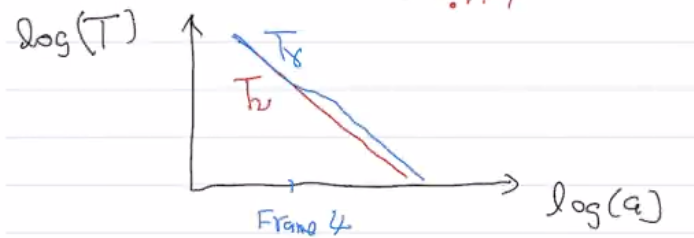
\includegraphics[width=0.75\textwidth]{entropy_transfer.png}
    \caption{Caption}
    \label{fig:my_label}
\end{figure}

What about protons and neutrons? We need more detailed thermodynamics here, but the result:

\be
\frac{n_n}{n_p} \sim 0.2
\ee

The main reaction here to form nuceli is $\text{p} + \text{n} \iff \text{D} + \underbrace{\gamma}_\text{2.2 MeV}$ since directly making He is incredibly unlikely. Are there enough reactions taking place? This is called the ''deuterium bottleneck,'' and we \textbf{must} break this bottleneck. Thus, $\text{D}$ is still unstable until $T$ drops further. 


\subsubsection{Frame 5: t = 3 minutes}

Here, we have $T_\gamma \sim 10^{9} \unit{K}$, giving $kT_\gamma = 0.086 \unit{MeV}$. Remember that $g^\star = 2$. Most of the positrons and electrons have disappeared, and we still have the \textbf{deuterium bottleneck}, so there are no appreciable heavier nuclei yet. Free neutron decay starts to become more important, and the neutron-proton ratio is:

\be
\frac{n_n}{n_p} \sim 0.16
\ee


\subsubsection{Frame 5.5: t = 3.75 minutes}

Here, we have:

\be
\frac{n_n}{n_p} \sim \frac17
\ee

This is when deuterium becomes stable enough for: $\text{n} + \text{p} \rightarrow \text{D} + \gamma$. \textbf{This is when nucleosynthesis begins}. Very quickly, nearly all neutrons turn into Helium-4. There are a few isotopes like tritium, He-3, and a bit of lithium. But, most of the neutrons are in Helium-4.

What is the helium abundance? Let $Y$ be the mass fraction of Helium:

\be
Y = \frac{4m_p n_{He-4}}{m_p n_{baryons}}
\ee

We also have $n_{He-4} = \frac{n_n}{2}$. Substituting that in:

\be
Y = \frac{2 \frac{n_n}{n_p}}{\frac{n_n}{n_p}}
\ee

For $n_n / n_p \sim 1/7$, we have $\boxed{Y = 1/4}$. 


There is one more thing to note. The BBN He abundance Y depends on a number of other basic parameters in addition to temperature in the Universe. Some of these include:

\begin{itemize}
    \item Baryon-to-photon ratio $\eta \equiv \frac{n_B}{n_\gamma} = \frac{n_n + n_p}{n_\gamma}$. We can show (in Problem Set 4): $\Omega_{0,B} h^2 = 0.00365 \eta_{10}$ where $\eta_{10} = \frac{\eta}{10^{-10}}$. Thus, if we can measure $\eta$, we can measure $\Omega_{0,B}$! If we have a larger $\eta$, deuterium is more stable and the bottleneck is broken earlier. Thus, we have a higher $Y$ for higher $\eta$. 
    \item Neutron lifetime: $\tau_n = 880.2 \pm 1.0 \s$ (2019) where $N(t) = N_0 e^{-t/\tau_n}$. If the neutron lifetime is longer, we have fewer neutron decays and thus higher $Y$. 
    \item Number of species of neutrinos $N_\nu$ (or $g^\star$ generally). Larger $N_\nu$ gives us larger $g^\star$. The net result is that we have a larger $Y$.  
\end{itemize}

\begin{figure}
    \centering
    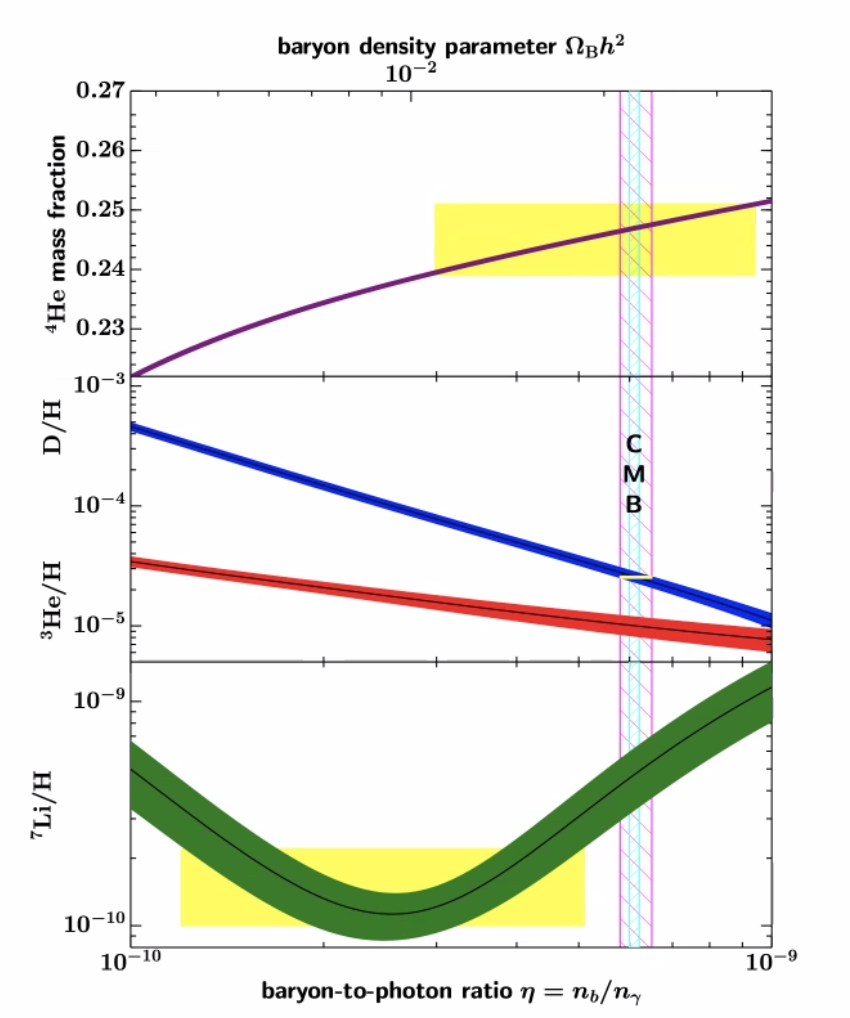
\includegraphics{Screen Shot 2021-03-10 at 11.51.46 AM.png}
    \caption{The master plot for discussions of BBN. This is from \url{https://pdg.lbl.gov/2020/reviews/rpp2020-rev-bbang-nucleosynthesis.pdf}. }
    \label{fig:lablablab}
\end{figure}


\section{The Mildly Lumpy Universe}

\subsection{Gravitational Instability in a Static Medium}

How does a \textit{nearly} smooth Universe become some lumpy? The basic principle is \textbf{gravitational instability}: tiny deviations from equilibrium become greatly enhanced. In practice, this means that \textbf{slightly overdense regions become denser}, whereas \textbf{slightly underdense regions become less dense}. How do we quantify this process? 

In the static case, we have the \textbf{Jeans Instability}. For a static Universe filled with non-relativistic fluid with mass density $\rho$, pressure $P$, (fluid) velocity $\vec{v}$, and gravitational potential $\Phi$. In this classical limit, what are the equations that govern these quantities?

Here are the fluid equations:

\noindent\textbf{Continuity Equation/Mass Conservation:}

\be
\partial_t \rho + \vec{\nabla} \cdot (\rho \vec{v}) = 0
\ee

\noindent\textbf{Equation of Motion (Euler Equation):}
\be
\underbrace{\partial_t \vec{v} + \left(\vec{v} \cdot \vec{\nabla}\right)\vec{v}}_\text{acceleration} = -\frac{1}{\rho}\vec{\nabla}P - \vec{\nabla} \Phi
\ee

Note that above, we are ignoring viscosity, magnetic fields, etc. We can include those on the right side of the Euler equation. 

\noindent\textbf{Poisson Equation:}
\be
\nabla^2 \Phi = 4\pi G \rho
\ee

We have three equations with four unknowns, so we need the equation of state for a unique solution. 

The unperturbed piece (with subscript $0$): static uniform fluid:

\be
\rho_0 = P_0 = \vec{v}_0 = \text{const.}
\ee

And we introduce small perturbations (like $\rho_1 \ll \rho_0$ with a subscript $1$ (which are not necessarily constant):

\be
\rho = \rho_0 + \rho_1
\ee

\be
P = P_0 + P_1
\ee

\be
\vec{v} = \vec{v}_1
\ee

\be
\Phi = \Phi_0 + \Phi_1
\ee

Let's introduce one other concept: sound speed. Specifically, we are talking about \textbf{adiabatic sound speed}:

\be
v_s^2 \equiv \left(\frac{\partial P}{\partial \rho}\right)_\text{const. entropy} = \frac{P_1}{\rho_1}
\ee

Note! If we don't have perturbations, we don't have a sound speed! We return to the master equations and we get two sets of equations -- perturbed and unperturbed. Starting with the zeroth-order fluid equations:

\noindent\textbf{Unperturbed Fluid Equations:}
\be
0 + 0 = 0
\ee

\be
\partial_t \vec{v}_0 + \left(\vec{v}_0 \cdot \vec{\nabla}\right)\vec{v}_0 = -\frac{1}{\rho_0} \vec{\nabla}P_0 - \vec{\nabla}\Phi_0 \rightarrow \Phi_0 = \text{const.}
\ee

\be
\nabla^2 \Phi_0 = 4\pi G\rho_0 \rightarrow \vec{\nabla} \Phi_0 = \frac{4\pi}{3} G\rho_0 \vec{r}
\ee

But we just said that the term had to be $0$! Historically, this is called \textbf{Jean's Swindle}: a basic inconsistency between Poisson and Euler equation. It's not worth doing, there is no reconciliation! Mathematically this checks out. What doesn't check out -- there is no such thing as a \textbf{static, uniform, fluid}. We are not allowing a pressure gradient to balance gravity, but we \textbf{NEED A PRESSURE GRADIENT TO BALANCE GRAVITY}. So, what's the swindle? We worry about this if it were relevant at all to physics; this is not the case since we never worry about it!

Any system with rotation, or any system that is not static, we don't have a Jean's swindle. Let's look at the \textbf{perturbed equations} to first order:

\be
\partial_t \rho_1 + \rho_0\vec{\nabla} \cdot \vec{v}_1 = 0
\ee

\be
\partial_t \vec{v}_1 = -\frac{v_s^2}{\rho_0}\vec{\nabla}P_1 - \vec{\nabla} \Phi_1
\ee

\be
\nabla^2 \Phi_1 = 4\pi G \rho_1
\ee

We can combine these since we have three equations with three unknowns (treating $v_s$ as a parameter):

Let's combine the first two perturbed equations (by taking the derivative of the first equation with respect to time and exchanging order of partials):

\be
\partial_t^2 \rho_1 + \rho_0 \left(-\frac{v_s^2}{\rho_0} \nabla^2 \rho_1 - \nabla^2 \Phi_1\right)
\ee

Using equation 3...

\be
\boxed{\partial^2_t  - v_s^2 \nabla^2 \rho_1 - 4\pi G \rho_0\rho_1 = 0}
\ee

This is the linearized fluid equation. It is functionally similar to the wave equation with a non-zero driving term. The standard trick is to go to Fourier space with an ansatz:

\be
\rho_1 (\vec{r},t) \propto \int e^{i(\vec{k}\dot\vec{r} - \omega t)} c\left(
\vec{k}\right) \mathrm{d}^3 k
\ee

This gives:

\be
-\omega^2 + v_s^2 k^2 - 4\pi G \rho_0 = 0 
\ee

\be
\boxed{\omega^2 = v_s^2 k^2 - 4\pi G \rho_0 }
\ee

This is the \textbf{dispersion relation for a linearized gravitational instability}. What is gravity doing here? The minus sign is crucial. Contrast this with the plasma frequency (which comes from electromagnetism which has \textit{two} signs):

\be
\omega^2 = v^2_s k^2 + \frac{4\pi n_e e^2}{m_e} > 0
\ee

What happens when $\omega^2 < 0$ in the gravitational case? Let's rewrite $\omega^2$:

\be
\omega^2 = v_s^2 \left(k^2 - k_J^2\right)
\ee

where we define the \textbf{Jeans wavenumber} and correspondingly a \textbf{Jeans' length} and a \textbf{Jeans' mass}:

\be
k_J \equiv \sqrt{\frac{4\pi G \rho_0}{v_s^2}}
\ee

\be
\lambda_J = \frac{2\pi}{k_J} = 2 \times \text{ Jean's Radius}
\ee

\be
M_J = \frac{4\pi}{3} \lambda_J^3 \rho_0
\ee

This last quantity gives us a scale for gravitational collapse.

Anyways, let's continue!

Naturally, we have two regimes:

\begin{itemize}
    \item $k > k_J$ or $\lambda < \lambda_J$. In this case, we have $\omega^2 > 0$ and $\omega$ is thus real. As a consequence, $\rho_1$ oscillates like sound waves! This is stable.
    \item $k > k_J$ or $\lambda > \lambda_J$. In this case, $\omega^2 < 0$, and $\omega \in \mathbb{C}$, giving us an exponential damping in time for the solution: $\rho_1 \propto e^{\pm |\omega|t}$. This grows or decays \textbf{exponentially}. This is \textbf{Jean's Instability}, or more generally, a \textbf{gravitational instability}. There are other instaiblities -- Kelvin-Helmholtz, Rayleigh-Jeans, etc. 
\end{itemize}

What are the underlying physics? Balance between pressure (outward) and gravity (inward). When pressure is larger, you get oscillations. When gravity is larger, we have an instability. 

By the way, let's do the SAME THING but much easier. This is called a \textbf{desert-island} analysis -- we are stuck on an island, and we need Jean's instability to get our boat moving. Let's start by looking at the dimensions of the forces and then the timescales:

\begin{enumerate}
    \item Instability occurs if gravity is larger than pressure, so consider the forces on a fluid element at the boundary of a star of density $\rho$ and radius $R$.
    \be
    \frac{F_G}{V_\star} \sim \frac{GM\rho}{R^2} \sim G R \rho^2
    \ee
    \be
    \frac{F_P}{V_\star} \sim \nabla P \sim v_s^2 \nabla \rho \sim v_s^2 \frac{\rho}{R}
    \ee
    \begin{itemize}
        \item Gravity wins if $F_G > F_P$
    \end{itemize}
    \be
    G \rho^2 R > \frac{v_s^2 \rho}{R} \rightarrow \boxed{R > \sqrt{\frac{v_s^2}{G \rho}} \sim \lambda_J}
    \ee
    
    \item Instability occurs if free-fall timescale (gravity) is smaller than sound crossing time:
    
    \be
    R \sim a_\text{accel.}t_g^2 \sim \frac{GM}{R^2} t_g^2 \sim G \rho R t^2_g
    \ee
    \be
    \boxed{t_g \sim \frac{1}{G\rho}}
    \ee
    \be
    t_p \sim \frac{R}{v_s}
    \ee
    \be
    t_g < t_p \rightarrow \frac{1}{\sqrt{G\rho}} < \frac{R}{v_s} \rightarrow R > \sqrt{\frac{v_s^2}{G\rho}}
    \ee
\end{enumerate}


\subsection{Gravitational Instability in an Expanding Medium}

James Jeans definitely did not know about this! 

Recall our fluid equations:

\be
\rho_0 = \rho_0(t) \text{ and } \rho_1 \equiv \delta \rho_0 \text{ where } \delta \equiv \frac{\rho - \rho_0}{\rho_0}
\ee

We introduced the ``fractional deviation'' $\delta$ from uniform background. The smallest $\delta$ can be is $-1$, but it has no bound! Just keep that in mind. We also have to take Hubble expansion into account:

\be
\vec{v}_0 = H \vec{r} = \frac{\dot{a}}{a} \vec{r}
\ee

And $\vec{v}_1$ is the peculiar velocity. One thing to note for later that we will need: $\vec{\nabla} \cdot \vec{v}_0 = \frac{\dot{a}}{a} \vec{\nabla} \cdot \vec{r} = 3 \frac{\dot{a}}{a}$.

Returning to our fluid equations:

\be
\partial_t \rho + \vec{\nabla} \left(\rho \vec{v}\right) = 0
\ee

To 0th order, 

\be
\frac{\partial \rho_0}{\partial t} + \rho_0 \vec{\nabla} \cdot \vec{v}_0  = \dot{\vec{\rho}}_0 + 3\frac{\dot{a}}{a} \rho_0 = 0 
\ee

Solving in our head...we get what we had seen earlier in class!

\be
\rho_0 \propt a^{-3}
\ee

The linearised (first order piece):

\be
\dot{\rho}_1 + \rho_0 \vec{\nabla} \cdot \vec{v}_1  + \vec{\nabla} \left(\rho_1 \vec{v}_0\right)
\ee

We can now switch to $\delta$ notation...

\be
\underbrace{\dot{\rho}_0 \delta}_{-3\dot{a}/a \rho_0}+ \rho_0 \dot{\delta} + \rho_0 \vec{\nabla} \cdot \vec{v}_1 + \rho_0 \vec{v}_0 \cdot \vec{\nabla} \delta + \underbrace{\rho_0 \delta \vec{\nabla} \cdot \vec{v}_0}_{3\dot{a}/a \rho_0} = 0
\ee

Simplifying....

\be
\boxed{\dot{\delta} + \vec{\nabla} \cdot \vec{v}_1 + \left(\frac{\dot{a}}{a}\vec{r} \cdot \vec{\nabla} \right)\delta}
\ee

The first term is the density change, the second term is a velocity flux, and the third term reminds us that we are in an expanding fluid.

Now take a look at the equation of motion:

To 0th order, 

\be
\frac{\partial \vec{v}_0}{\partial t} + \left(\vec{v}_0 \cdot \vec{\nabla}\right)\vec{v}_0 = -\vec{\nabla} \Phi_0 \neq 0 \text{ unlike the static case}
\ee

There is no Jeans Swindle here! Now to first order, we get...

\be
\partial_t \vec{v}_1 + \left(\vec{v}_0 \cdot \vec{\nabla}\right) + \left(\vec{v}_1 \cdot \vec{\nabla}\right)\vec{v}_0 = -\frac{v_s^2 \vec{\nabla} \rho}{\rho_0} - \vec{\nabla} \Phi_1
\ee

Note:

\be
\left(\vec{v}_1 \cdot \vec{\nabla} \right) \vec{v}_0 = H \left(v_{1x} \partial_x + v_{1y} \partial_y + v_{1z} \partial_z\right)\vec{r} = H \vec{v}_1 = \frac{\dot{a}}{a} \vec{v}_1
\ee

This makes:

\be
\boxed{\partial_t \vec{v}_1 + \frac{\dot{a}}{a} \left(\vec{r} \cdot \vec{\nabla}\right)\vec{v}_1 + \frac{\dot{a}}{a}\vec{v}_1 = - v_s^2 \vec{\nabla} \delta - \vec{\nabla} \Phi_1}
\ee

The last is trivial:

\be
\boxed{\nabla^2 \Phi_0 = 4\pi G \rho_0 \text{ and } \nabla^2 \Phi_1 = 4\pi G \rho_0 \delta}
\ee










\appendix 

\section{Archival Lectures (C.P. Ma)}

\subsection{Lecture 1}

\subsubsection{ The Cosmological Principle}

The {\bf Cosmological Principle} states that the universe is spatially 
{\it isotropic} (looks the same in all directions) 
and {\it homogeneous} (has constant density everywhere) on large scales.
The {\bf Perfect Cosmological Principle} states that the universe is
also {\it temporally} isotropic and homogeneous (a steady state universe). 
This is unlikely because it doesn't describe the Cosmic Microwave Background
(CMB).  The CMB and Hubble's Law are both provide evidence for isotropy and
homogeneity.

\subsubsection{ Hubble's Law (1929) }

Hubble's Law is an empirical law stating that, on large scales, recessional 
velocity is proportional to distance from observer.
$$\boxed{v=Hr}$$ 
where $H$, the Hubble parameter, is not constant, but can
vary slowly with time.  By convention, $H$ is often expressed as
$H=100\cdot h\frac{km}{ s\cdot Mpc}$, where 1 parsec (pc) $\approx3\cdot10^{18}cm
=3.26ly$, is the distance at which 1 AU appears as 1 arcsec on the sky.  
The Hubble Space Telescope Key Project (Freedman et al. ApJ 553, 47, 2001)
measured the present day value of Hubble Constant 
$H_0=72\pm 8\frac{km}{ s\cdot Mpc}$, giving us that the current timescale for
the expansion of the universe is 
$H_0^{-1}\approx\frac{h}{ 10^{11}}yrs\approx 9.778h^{-1}Gyrs$.

\subsubsection{ The Scale Factor }

$a(t)$ relates physical ($r$) and {\it comoving} ($x$) coordinates in an
expanding universe:
\begin{align}
r&=a(t)x\\
\dot r&=\dot ax+a\dot x=\underbrace{\aa}_{\equiv H}r+\underbrace{a\dot x}_{\equiv v_p}\\
\end{align}
Thus, the two components of physical velocity are $H$ (the Hubble expansion 
parameter) and $v_p$ (the peculiar velocity, or motion relative to expansion)
By convention, $t_0 \equiv$ today and $a(t_0)=1$.

\subsubsection{ The Friedmann Equations}

The Friedmann Equation is an equation of motion for $a(t)$.  A rigorous
derivation requires General Relativity, but we can fake it with a
quasi-Newtonian derivation.
We will model the universe as an {\it adiabatically} ($\Delta S=0$) expanding,
isotropic, homogeneous medium.  Isotropy allows us to use $r$ as a scalar.
Consider a thin, expanding spherical shell of radius $a$.
Birkhoff's Theorum states that even in GR,
the motion of such a shell depends only on the enclosed mass 
$M={4\pi }{ 3}a^3\rho$.
Thus, the energy per unit mass per unit length is:
$$E=\overbrace{\hf \dot a^2}^{Kinetic}\overbrace{-\frac{G\cdot M}{ a}}^{Potential}
=\hf \dot a^2-\frac{4\pi }{ 3}G\rho a^2.$$
We define $k\equiv-\frac{2E}{ c^2}$, and we will show later that $k$ is a measure
of the curvature of the universe: 
$$k\begin{cases}
>0&\,for\ E<0\ (bound)\\
=0&\,for\ E=0\ (critical)\\
<0&\,for\ E>0\ (unbound)\\\end{cases}$$
where $k$ has units of $\inv{length^2}$ if $a$ is dimensionless.  Substituting
$k$ into the above energy equation, and solving for $\aa$, we get:
\def\paap{\left(\aa\right)}
$$\boxed{H^2=\paap^2=\epot G\rho -\frac{k c^2 }{ a^2}}$$
\centerline{($1^{st}$ Friedmann Equation)}
This is a statement of conservation of $E$.
The first law of thermodynamics ($\Delta S=0$) requires that any 
system with positive pressure must lose energy as the volume enclosing it
expands.  Thus, if $U$ is our internal energy and $P$ is our pressure:
$$\frac{dU}{ dt}=-P\frac{dV}{ dt}.$$  
In an expanding universe, $U={E}{ V}\cdot V=\rho a^3$, where $\rho$ is the
energy density of the universe.  $P$ is the pressure of the photon gas, so:
$$\dot \rho a^3+3\rho a^2\dot a=-P 3a^2\dot a,$$ 
which simplifies to:
$$\boxed{\dot \rho=-3\aa(\rho +P)}$$
\centerline{($2^{nd}$ Friedmann Equation)}
This is a a statement of the temperature loss of the universe 
due to adiabatic expansion.\par
Finally, $\ddt$($1^{st}$ Friedmann Equation) gives us:
$$2\dot a\ddot a=\epot G \frac{d }{ dt}(\rho a^2) =\epot G a^2(\dot \rho +2\aa \rho).$$
Substituting the $2^{nd}$ Friedmann Equation for $\dot \rho$:
$$2\dot a\ddot a=\epot Ga^2 (-\aa \rho -3 \aa P) =-\epot G \aa (\rho +3P).$$  
Now we have our $3^{rd}$ Equation:
$$\boxed{\frac{\ddot {a }}{ a}=-\frac{4\pi G} {3} (\rho + 3P)}$$
\centerline{($3^{rd}$ Friedmann Equation)}
The $3^{rd}$ Friedmann Equation relates the acceleration of the expansion of
the universe to the pressure of photon gas and the density of the universe.
Note that if $3P \le -\rho$, we have an accelerating universe.\par
Compare the $3^{rd}$ Friedmann Equation to the Newtonian equation for gravity,
with $M=\frac{4\pi }{ 3}\rho x^3$ and $\rho_{eff}=\rho +3P$:
$$\ddot x=\frac{-G\cdot M}{ x^2}={-4\pi }{ 3}G\rho x$$

\subsection{Lecture 2}

\subsubsection{ The Friedmann Equations, continued }

Recall we had the following equations:
$$\paap^2={8\pi}{3}G\rho-\frac{k}{ a^2}$$
$$\dot \rho=-3\aa(\rho+P)$$
$$\frac{\ddot a}{ a}=-\frac{4\pi}{3}G(\rho+3P)$$

To close the equations, we need to relate $P$ and $\rho$ with an equation of
state:
$$\boxed{P=w\rho(c^2)}$$ 
Note that we will generally set $c=1$ in this class.
Combined with (2), this gives us:
\begin{align}
\dot \rho&=-3\aa(1+w)\rho\\
{\dot \rho}{\rho}&=-3(1+w)\aa\\
\rho&\propto\atow\\
\end{align}
Note that we've assumed $\dot w=0$, which is okay most of the time.
Some special cases of interest are:
\begin{itemize}
\item Pressure-less ``dust'' $P=0$, $w=0\imply\rho\propto a^{-3}$ because volume
goes as $V\propto\inv{a^3}$.
\item Relativistic particles (photons, bosons): $w=\inv{3}$, $P=\frac{\rho}{3}
\imply\rho\propto a^{-4}$ because $VV\propto\inv{a^3}$, and energy is given
by $E\propto\inv{a}$.
\item  ($\Lambda$)/Dark Energy: $w=-1$, $P=-\rho\imply\rho=$ constant 
in time.
\end{itemize}
To get density ($\rho$) as a function of time, want to solve for $w$.

\subsubsection{ Critical Density}

We define $\rho_{crit}$ to be the critical density at which $k=0$ (and $E=0$):
\def\rcr{{\rho_{crit}}}
$$\rcr=\frac{3H^2}{8\pi G}$$
Today, we measure: $\rho_{crit,0}=\frac{3H_0^2}{8\pi G}= 
\frac{3}{8\pi}\frac{\left(100h\frac{km}{ sMpc}\right)^2}{ G}=2.78\cdot10^{11}h^2
\frac{M_\odot}{ Mpc^3}=1.88\cdot10^{-29}h^2\frac{g}{ cm^3}$.
Note that the mass of the sun is $M_\odot=2\cdot10^{33}g$, and
the mass of the proton is $M_p=1.67\cdot10^{-24}g$.

\subsubsection{ Density Parameter}

$\Omega$ measures the ratio of the density of the universe to the critical
density:
$$\Omega(t)\equiv\frac{\rho(t)}{\rho_c(t)}=\frac{8\pi G\rho(t)}{ 3H^2(t)}$$
$$\Omega\begin{cases}
\le1&\imply open\ (k\le0)\\
=1&\imply flat\ (k=0)\\
\ge1&\imply closed\ (k\ge0)
\end{cases}$$

In general, $\Omega$ can consist of multiple components: 
$\Omega=\sum_i{\Omega_i}$ e.g. 
$$\Omega\begin{cases}
r&=radiation\\ 
m&=matter\ (dark\ and\ luminous)\\
b&=baryons\ (dark\ and\ luminous)\\ 
\nu &=neutrinos\\ 
\Lambda&=dark\ energy\end{cases}$$

$\Omega = 1$ is an unstable equilibrium; any perturbation from $\Omega=1$ in
the early universe ensures $\Omega$ is far from 1 today.  That we measure
$\Omega_m\approx0.3$ today implies that the early universe must have been
extremely finely tuned.

\subsubsection{ Evolution of Hubble Parameter}

Today (at $a=1$): $k=\epot G\rho_0-H_0^2=H_0^2(\Omega_0-1)$.  Using the
$1^{st}$ Friedmann equation (1), we have:
$$\boxed{H^2=H_0^2(\frac{\Omega_0}{ a^{3+3w}}+\frac{1-\Omega_0}{ a^2})}$$
\centerline{\bf (THE Friedmann Equation)}
where $H_0\equiv\sqrt\frac{8\pi G\rho}{3\rcr}$, and it is understood that
$\etot=\sum_i{\Omega_{i,0}}$.  Each $\Omega_i$ has it's own $w_i$, so really
$\frac{\Omega_0}{\attw}=\sum_i\frac{\Omega_{i,0}}{ a^{3+3w_i}}$.

\subsubsection{ Evolution of Density Parameter}

We'll show in PS\#1 that for any single component:
$$\frac{1-\Omega(a)}{\Omega(a)}=\frac{1-\Omega_0}{\Omega_0}a^{1+3w}$$
Plotting $\Omega(a)$, we will find that for early $a$, $\Omega$ is {\it 
extremely} close to 1.

\subsubsection{ Evolution of Scale Factor: Solving the Friedmann Equation}

The evolution of the expansion of the universe is governed by:
$$\paap^2=\epot G\rho-\frac{k}{ a^2}$$

We can apply this to several models of the universe:
\begin{itemize}
\item The Einstein-deSitter (flat) Model: $k=0$, $\Omega(a)=\Omega_0=1$.
Using that $\rho\propto\atow$, we have:
\begin{align}
\paap^2&\propto\atow\\
a^{-1}a^{\frac{3}{ 2}(1+w)}da&\propto dt\\
\athow&\propto t\\
\end{align}$$
$$\boxed{a(t)\propto t^{\frac{2}{ 3(1+w)}}}
Thus, the rate of expansion of the universe depends on $w$:
\item{(a)} The matter-dominated era: 
$\Omega\approx\Omega_m\imply w=0, P=0, a\propto t^\frac{2 }{ 3}$.
\item{(b)} The radiation-dominated era: 
$\Omega\approx\Omega_r\imply w=\inv{3} \imply a(t)\propto t^\hf$.
\item{(c)} The $\Lambda$-dominated era: 
$\Omega\approx\Omega_\Lambda\imply w=-1, P=-\rho, \rho$ constant in time
$\imply a(t)\propto e^{Ht}$, where H is now actually a constant.  This
is exponential inflation.  We used to think that this only happened early on 
(like $10^{-34}$
seconds), but now we think that this has also been happening recently.
Next time, we will do the harder two cases: open and closed.
\end{itemize}

\subsection{Lecture 3}

\subsubsection{ Evolution of Scale Factor: Solving the Friedmann Equation, continued }

Last time we did (1), the flat universe:

Einstein-deSitter, $k=0$ (flat), $\Omega =1,\imply$
 $a\propto t^\frac{2}{ 3(1+w)}$. In general, we consider the evolution of
the universe to be {\it matter dominated} if $a\propto t^\frac{2}{ 3}$,
{\it radiation dominated} if $a \propto t^{\hf}$, and 
{\it $\Lambda$ dominated} if $a \propto e^{1+t}$ (that is, $H$ is constant).


Open, $k<0$, $\etot<1$, $\econs=0$, $\emat<1\imply$ our Friedmann
Equation $\paap^2=\epot G\rho-\frac{k}{ a^2}$ becomes:
$$\dot a^2=H_0^2\left(\frac{\etot }{ a^{1+3w}}+1-\etot\right)$$  
Since we are matter dominated, $w=0$.  Solving for $a(t)$:
\begin{align}
\int_0^{a_f}\frac{da}{\sqrt{{\etot}{ a}+1-\etot}}
&=\int_0^{t_f}{H_0\cdot dt}\\
\int_0^{a_f}\frac{a\cdot da}{\sqrt{1-\etot}\sqrt{a^2+\frac{\etot}{1-\etot}a}}
&=H_0t_f\\
\end{align}
Let's define $2\alpha\equiv\frac{\etot}{1-\etot}$.  Then:
$$\int_0^{a_f}\frac{a\cdot da}{\sqrt{1-\etot}\sqrt{(a+\alpha)^2-\alpha^2}}
=H_0t_f$$
Defining $a^\prime=a+\alpha$, we get:
\begin{align}
\int_0^{a_f+\alpha}\frac{(a^\prime-\alpha)da^\prime}{ 
\sqrt{1-\etot}\sqrt{a^{\prime 2}-\alpha^2}}&=H_0t_f\\
\int_0^{a_f+\alpha}\frac{(a-\alpha)da}{ \sqrt{1-\etot}\sqrt{a^2-\alpha^2}}
&=H_0t_f\\
\end{align}
Now we define $\alpha\cosh\theta\equiv a^\prime$, 
$\alpha\sinh\theta\,d\theta=da$, so that 
$\sqrt{a^{\prime 2}-\alpha^2}=\alpha\sinh\theta$.  We'll be lazy and
just say that $a_f^\prime\to\frac{\etot }{ 2(1-\etot)(\cosh\theta -1)}$ because
there was nothing special about time $a_f^\prime$. Then we have:
\begin{align}
\int_0^{\theta_f}\frac{\alpha^2(\cosh\theta-1)\sinh\theta\,d\theta}{
\sqrt{1-\etot}\alpha\sinh\theta}&=H_0t_f\\
\frac{\alpha}{1-\etot}(\sinh\theta-\theta)\bigg|_0^{\theta_f}&=H_0t_f\\
\end{align}

Plugging $\alpha$ back in:
\begin{align}
H_0t_f&=\frac{\etot}{2(1-\etot)^\frac{3}{ 2}}(\sinh\theta-\theta)\\
t(\theta)&=\frac{\etot}{2H_0(1-\etot)^\frac{3}{2}}(\sinh\theta-\theta)\\
\end{align}
Thus we have a parametric relationship between $a$ and $t$ with a dummy
variable $\theta$:
\begin{align}a(\theta)&=\frac{\etot}{ 2(1-\etot)}(\cosh\theta-1)\\
t(\theta)&=\frac{\etot}{ 2\,H_0(1-\etot)^{3}{ 2}}(\sinh\theta-\theta)\\
\end{align}
Note that $a$ has no maximum and expands forever.

Closed, $k>0$, $\etot>1$, $\Omega_\Lambda=0$. As usual,
we start with the Friedmann Equation:
$$(\aa)^2 = \underbrace{\overbrace{\epot G\rho}^{positive} - 
\overbrace{\frac{k}{ a^2}}^{positive}}_{can\ be\ 0}$$
Therefore, in this model it is possible for $\dot a=0$.  We'll again solve for a
matter-dominated era, $w=0$.  The solution is similar, to the open model, 
but ($1-\etot<0$), so $\theta\to i\,\theta$. Thus our solution:
\begin{align}a(\theta)&=\frac{\etot}{ 2(1-\etot)}(\cos\theta-1)\\
t(\theta)&=\frac{\etot}{2H_0(1-\etot)^\frac{3}{ 2}}(\sin\theta-\theta)\\
\end{align}
is a cycloid solution.  That is, $a$ oscillates, with a maximum at 
$\theta=\pi$.

\subsubsection{ Deceleration Parameter q}

$$q\equiv-{\ddot aa}{ \dot a^2}$$
Note that $q$ is {\it dimensionless}, and has a negative sign.  The minus is
there because historically, the universe was thought to be decelerating.  Thus,
$q<0\imply acceleration$, and $q>0\imply deceleration$.  We can find out what
$q$ does from the $2^{nd}$ Friedmann Equation:
$$\adda=-\frac{4\pi}{3}G(\rho+3P)$$
Recall that $P=w\rho$, $\Omega=\frac{\rho}{\rcr}$,
$\rcr=\frac{3H^2}{8\pi G}$, $H^2\Omega=\epot G\rho$. Thus, the
above equation becomes:
$$\adda=-\frac{4\pi}{3}G\rho(1+3w)=-\frac{H^2\Omega}{2}(1+3w)$$
Substituting in our friend, $q$:
$$q=\frac{\Omega}{2}(1+3w)=\sum_i{\frac{\Omega_i}{2}(1+3w_i)}$$
$$\boxed{q = \frac{\Omega _m }{ 2} - \Omega _\Lambda +\Omega _r}.$$
Note that today, $\Omega_r\ll1$.  That we are accelerating $\imply q<0
\imply\econs\ne0$.

\subsubsection{ Redshift }

$$\frac{\lambda_{obs} }{ \lambda_{emit}} \equiv 1 + z$$
Or alternately,
$$\boxed{1 + z = \frac{1}{ a}}$$
$z$ is what we call the {\it redshift}. Reionization happened somewhere
around $z=17\pm6$, and recombination around $z=1091$.

\subsubsection{ Time-Redshift Relations and the Age of the Universe }

We seek a relation between $t$ and $z$.  Beginning with the Friedmann Equation:
\begin{align}
H^2&=H_0^2\left[\jumble\right]\\
\inv{a}\frac{da}{ dt}&=H_0\sqrt{\jumble}\\
dt&=\inv{H_0}\left(\inv{a}\right)\frac{da}{\sqrt{\jumble}}\\
dt&=-\inv{H_0}\frac{dz }{ (1+z)\jimble}\\
\end{align}
We can calculate the time since the Big Bang at redshift $z_1$ by solving the
integral:
$$t_1=-\inv{H_0}\int_{z_1}^\infty{\frac{dz}{ 1+z}\inv{\jimble}}$$
For the Age of the Universe, set $z_1=0$.  In the special case of a flat
(Einstein-deSitter) universe: 
$$t_0=\inv{H_0}\int_0^\infty\frac{dz}{(1+z)^\frac{5}{ 2}}={2}{3H_0}$$  
If $H_0^{-1}\approx10Gyrs$,
then $t_0\approx6.7h^{-1}Gyrs$, so the Hubble constant needs to be pretty
small to get reasonable estimates of the age of the universe.



\subsection{Lecture 4}

\subsubsection{ Time-Redshift Relations and the Age of the Universe }

Last time we found the age of a flat universe.
in a flat (Einstein-deSitter) universe: 
$k=0$, $\Omega_m=1$, $\Omega_\Lambda=0$, so:
$$t_0=\inv{H_0}\int_0^\infty{\frac{dz}{(1+z)^\frac{5}{ 2}}}
=\frac{2}{3H_0}\approx6.7h^{-1}Gyr$$
Alternatively, recall that for a matter-dominated era,
$a(t) = ({t}{ t_0})^\frac{2}{ 3}.$
Thus, $H = \aa = \frac{2}{ 3t} \imply t_0=\frac{2}{ 3H_0}$.

If we have $\Lambda\ne0$: $k=0$, $\emat+\econs=1$, then:
$$t_0=\inv{H_0}\int_0^\infty\frac{dz}{(1+z)\sqrt{\emat(1+z)^3+\econs}}$$
Assuming $0.1\le\emat\le1$, this integral is solvable:
$$t_0=\frac{2}{3H_0}\inv{\sqrt{1-\emat}}\ln\left(\frac{1+\sqrt{1-\emat}}{
\sqrt{\emat}}\right)\approx\frac{2}{3H_0}(0.7\emat+0.3-0.3\econs)^{-0.3}
\approx\frac{2}{3H_0}\emat^{-0.3}$$
Generally, in a flat universe, $t_0\propto\inv{H_0}$.  If $\Omega_0\le1$, 
it will be longer.

In an open universe: $k<0$, $\etot<1(\econs=0)$. Recall:
$$\begin{matrix} t(\theta)=\frac{\etot}{2H_0(1-\etot)^\frac{3}{2}}(\sinh\theta-\theta),&
a(\theta)=\frac{\etot}{2(1-\etot)}(\cosh\theta-1)\end{matrix}$$

So today: 
\begin{align}
a(\thnot)&={\etot}{ 2(1-\etot)}(\cosh\thnot -1)=1\\
\cosh\thnot&=\frac{2(1-\etot)}{\etot}+1=\frac{2-\etot}{\etot}\\
\sinh\thnot&=\sqrt{\cosh^2\thnot-1}=\frac{2}{\etot}\sqrt{1-\etot}\\
t_0&=t(\thnot)-\frac{\etot}{ 2H_0(1-\etot)^\frac{3}{ 2}}\left[\frac{2}{\etot}
\sqrt{1-\etot}-\cosh^{-1}\left(\frac{2-\etot}{\etot}\right)\right]\\
\end{align}

$$\boxed{t_0=\inv{H_0}\left[(1-\etot)^{-1}-\hf(1-\etot)^{-\frac{3}{ 2}}
\cosh^{-1}\left(\frac{2-\etot}{\etot}\right)\right]}$$

Thus $t_0>\frac{2}{ 3H_0}$ for $\etot\le 1$, and $t_0=\inv{H_0}$ for $\etot=0$
(an empty universe).

In a closed universe: $k>0$, $\etot>1$, $(\econs=0)$. Recall: 
\begin{align}
t(\theta)&=\frac{\etot}{ 2H_0(\etot -1)^\frac{3}{2}}(\theta-sin\theta)\\
a(\theta)&=\frac{\etot}{ 2(\etot -1)}(1-\cos\theta)\\
\end{align}

Thus, today:
$$a(\theta_0)=\frac{\etot}{ 2(\etot -1)}(1-\cos\theta)=1$$
$$\boxed{t_0=\inv{H_0}\left[(1-\etot)^{-1}+\hf\etot(\etot-1)^{-\frac{3}{ 2}}
\cos^{-1}\left(\frac{2-\etot}{\etot}\right)\right]}$$

\subsubsection{ The Robertson-Walker Metric}

Lorentz invariance dictates that two inertial
frame $(x, y, z, t)$ and $(x\p, y\p, z\p, t\p)$, with one 
moving with respect to the other at velocity $\hat v=v\hat x$, are related by:
$$\begin{matrix} x\p=\gamma(x-vt),&y\p=y,&z\p=z,&t\p=\gamma\left(t-\frac{v}{ c^2}x
\right)\end{matrix}$$
where $\gamma\equiv\frac{1}{\sqrt{1-\frac{v^2}{ c^2}}}$.  
Note, to give a taste of tensor forms, this all
may be written as ${x\p}^\alpha = \Lambda^\alpha_\beta x^\beta+I_0^\alpha$.\par

Remember the Lorentz invariant interval, which is conserved between frames:
$$ds^2=c^2dt^2-(dx^2+dy^2+dz^2)$$
Light travels a $ds^2=0$ path.  In tensor form, this equation looks like:
$$ds^2=g_{\alpha\beta}dx^\alpha dx^\beta$$
where $g_{\alpha\beta}$, the metric tensor, is given by:
$$g_{\alpha\beta}\equiv\begin{pmatrix} 1&0&0&0\\0&-1&0&0\\0&0&-1&0\\ 0&0&0&-1\\
\end{pmatrix}$$
Look at Weinberg, Ch. 13 for full proof, but for a homogeneous, 
$\gamma$-isotropic space, the metric looks like: 
$$ds^2=c^2dt^2-a^2(t)\left[\frac{dr^2}{ 1-kr^2}+r^2d\Omega\right]$$
where $r$ is a radial direction (in
comoving coordinates), and $d\Omega=d\theta^2+\sin^2\theta d^2\phi$ is the
differential angle seperation of two points in space.  As usual,
$k$ is the measure of curvature.


The $k=0$ Model: 
$$dr^2+r^2(d\theta^2+\sin^2\theta d\phi^2)=dx^2+dy^2+dz^2$$
so we recover the Minkowski metric for flat space, using comoving coordinates.

The $k>0$ (closed) Model:\par
We get a coordinate singularity at $r=\frac{1}{\sqrt{k}}$, so this universe
has a finite volume.
For $k>0$, we need to define ``Polar Coordinates'' in 4-D (to describe a
3-sphere embedded in 4-D).  Here is a comparison of how we define polar 
coordinates for a 3-sphere in 4-D versus for a 2-sphere in 3-D:
$$\begin{matrix} 
3-sphere&2-sphere\\
(x,y,z,w)\iff (R,\alpha,\beta,\gamma)&(x,y,z)\iff(R,\theta,\phi)\\
w=R\cos\alpha&z=R\cos\theta\\
z=R\sin\alpha\cos\beta&y=R\sin\theta\cos\phi\\
y=R\sin\alpha\sin\beta\cos\gamma&x=R\sin\theta\sin\phi\\
x=R\sin\alpha\sin\beta\sin\gamma& \\
x^2+y^2+z^2+w^2=R^2&x^2+y^2+z^2=R^2\\
\end{matrix}$$

Take a line element on a 2-sphere: 
$$d\gamma=R^2(d\theta^2+\sin^2\theta d\phi^2)$$
Changing variables for $v\equiv\sin\theta$:
$$dv=\cos\theta d\theta=\sqrt{1-v^2}d\theta$$
Then $d\theta^2=\frac{dv^2}{1-v^2}$, so rewriting our line element, we get:
$$d\gamma^2=R^2\left(\frac{dv^2}{ 1-v^2}+v^2d\phi^2\right)$$
For a 3-sphere, 
$$d\gamma^2=R^2(d\alpha^2+\sin^2\alpha d\Omega^2)$$
where $d\Omega^2\equiv d\beta^2+\sin^2\beta d\gamma^2$.  Again, using a change
of variables so that $v\equiv\sin\alpha$, $d\alpha=\frac{dv}{\sqrt{1-v^2}}$,
we get that:
$$\boxed{d\gamma^2=R^2\left(\frac{dv^2}{ 1-v^2}+v^2d\Omega^2\right)}$$
This is what Robertson-Walker showed. 


\subsection{Lecture 5}

\subsubsection*{ Finishing the Robertson-Walker Metric}

We've been following Weinberg's derivation to show there are discrete metrics.
We'll start with:
$$ds^2=c^2dt^2-a^2(t)\left[\frac{dr^2}{ 1-kr^2}+r^2(d\theta^2+\sin^2\theta 
d\phi^2)\right]$$
Recall that $k$ is the {\it curvature constant} and $r$ is in {\it comoving}
coordinates.  If we define $U\equiv\sinh\theta$, then: 
\begin{align}
dU&=\cosh\theta\cdot d\theta\\
d\theta&=\frac{dU}{\sqrt{1+U^2}}\\
\end{align}
The beauty of this metric
is that we derived it only using symmetry (no dynamics).  There is an alternate
way of writing the metric above:
$$ds^2=c^2dt^2-a^2
\left[d\chi^2+S^2(\chi)(d\theta^2+\sin^2\theta d\phi^2\right]$$
where:
$$S(\chi)\equiv\begin{cases}\chi &\,(for\ k=0,\ \chi=r)\\
k^{-\hf}\sin(k^\hf \chi)&\,(for\ k>0)\\
(-k)^{-\hf}\sinh(\sqrt{-k}\chi)&\,(for\ k<0)\\\end{cases}$$
\par

\subsubsection*{ Comoving Radial Distance vs. Redshift: the Hubble Diagram }

This is the fundamental diagram behind using a standard candle (supernova) to
infer the curvature of the universe.  What we want here is an algebraic
expression relating $r$ and $z$.  We'll look at light propagation ($ds^2=0$),
and take a radial path ($d\theta=d\phi=0$) to know from the Robertson-Walker
metric that:
$$c^2dt^2=a^2\frac{dr^2}{1-kr^2}$$
Separating out our $r$ dependencies
and our $t$ dependencies and integrating, we get:
$$\int_0^{r_1}\frac{dr}{\sqrt{1-kr^2}}=\int_{t_1}^{t_0}\frac{c\cdot dt}{ a(t)}$$
\begin{itemize}
\item For the flat, $k=0$, matter-dominated model ($w=0$, $\econs=0$, 
$\emat=1$), we'll start with the Friedmann Equation:
$$H=\aa=H_0\sqrt{\frac{\etot}{\attw}+\frac{1-\etot}{ a^2}}$$
Recognizing that $a=\inv{1+z}$, we have:
$$H_0dt=-\frac{dz}{ (1+z)\sqrt{\etot(1+z)^{3+3w}+(1-\etot)(1+z)^2}}$$
These integrals evaluate to (in comoving $r$):
$$r_1=\int_{t_1}^{t_0}\frac{c\cdot dt}{ a(t)}$$
$$\boxed{r_1=\frac{2c}{ H_0}\left[1-(1+z)^{-\hf}\right]}$$
\def\hubd{\frac{2c}{ H_0}}
\def\sqmk{\sqrt{-k}}
Here, $\hubd$ is called the Hubble distance and is the definition of 
how far away we can possibly see--how far light could have traveled since the
beginning of time.  Notice that as $z\to\infty$, $r=\hubd\approx10000h^{-1}Mpc$.

\item For the open, $k<0$, $\etot<1$, $w=0$ model, we'll substitute 
$\sqmk r=\sinh\chi$, $dr=\frac{\cosh\chi d\chi}{\sqmk}$ for $r$ in the integral 
above:
\begin{align}
r&=\int_-^{\chi_1}\frac{\cosh\chi d\chi}{\sqmk\sqrt{1+\sinh^2\chi}}\\
\frac{\chi_1}{\sqmk}&={\sinh^{-1}(\sqmk r_1)}{\sqmk}\\
\end{align}
From this, we can use {\it Mattig's Formula}, which states for $w=0$, 
arbitrary $\emat = \etot$, that:
$$r=\frac{2c}{ H_0\etot^2}\inv{1+z}\left[\etot z+(\etot-2)(\sqrt{1+\etot z}
-1)\right]$$
In general, for arbitrary $\emat, \econs$ (we'll derive this in PS\#3), one
can show that, in comoving $r$:
\def\sqak{\sqrt{|k|}}
$$
\boxed{r=\inv{\sqak}sinn\left(\frac{c}{ H_0}\sqak 
\int_0^z\frac{dz\p}{ \sqrt{\emat(1+z)^3+\econs+(1-\emat-\econs)(1+z)^2}}
\right)}$$
where $sinn$ is a funny function: 
$$sinn\equiv\begin{cases}\sin&\,for\ k>0\\
absent&\,for\ k=0\\
\sinh&\,for\ k<0\\\end{cases}$$
Note that when $w=0$, for arbitrary $\emat$, we recover Mattig's Formula.
\end{itemize}

\subsubsection*{ Angular Diameter Distance}

The angular diameter distance is a useful quantity which relates the physical
size or separation of objects to the angular size on the sky.  For normal,
Euclidean geometries, this is trivial trigonometry.  For a curved universe,
this is not trivial.  For example, in some universes, an object pulled
far enough away may actually start looking larger (have a larger angular
diameter) than a closer object!\par
This brings us to the end of the smooth universe.  We've seen $a(t)$, but we
have not seen any perturbations off of that.  Similarly, we've seen $\rho (t)$,
but no spatial components of density.  We will begin to talk about perturbations
off of the Smooth Universe, and we will call this:

\subsubsection*{ The Bright Side of the Universe}

Let's do a quick tour of the the particles out there to give some context
to what we're talking about.  Take a look at {\it Review of Particle Physics},
which is also at {\it http://pgd.lbl.gov}, for some more detailed information.
\par
First, we'll talk about {\it fermions}.  Fermions come in two varieties:
Leptons and Quarks.  Quarks are hadrons and group together to from
baryons (made of 3 quarks) and mesons (made of quark-antiquark pairs).
\centerline{Elementary Particles: Fermions (spin $\hf$)}
$$\begin{matrix} 
Leptons&Charge&Mass&Mean\ Lifetime\\
e&-1&0.51099892\pm0.00000004 MeV&\infty\\
\nu_e&0&<3 eV&\infty\\
\mu&-1&106 MeV&2.2\mu s,\ \mu^-\to e^-\bar \nu_e\nu_p\\
\nu_\mu&0&<190 keV&\infty\\
\tau&-1&1.78 GeV&2.9\cdot 10^{-13}\\
\nu_\tau&0&<18.2 MeV&\infty\\\end{matrix}$$

$$\begin{matrix} 
Quarks\ (3\ colors\ each)&Charge&Mass\\
U&\frac{2}{ 3}&1.5 \to 4 MeV\\
d&-\frac{1}{ 3}&4 \to 8 MeV\\
s&-\frac{1}{ 3}&80 \to 130 MeV\\
c&\frac{2}{ 3}&1.15 \to 1.35 GeV\\
b&-\frac{1}{ 3}&4.1 \to 4.4 GeV\\
t&\frac{2}{ 3}&174.3 \pm 5.1 GeV\\\end{matrix}$$


\subsection{Lecture 6}

\subsubsection*{ The Bright Side, continued }

$$\begin{matrix} 
Gauge\ Bosons&spin&charge&mass\\
\gamma&1&0&0&(carries\ electroweak\ force)\\
w^\pm&1&\pm 1&80.4 GeV&(carries\ electroweak\ force)\\
Z^0&1&0&91.2 GeV&(carries\ electroweak\ force)\\
gluons&1&0&don't\ know&(carries\ strong\ force)\\
Higgs&0&0&>114.4GeV\\
graviton&2&0&0\\\end{matrix}$$

$$\begin{matrix} 
Baryons&quark\ content&charge&mass&lifetime\\
proton&uud&+1&938.07003 MeV&\ge 10^{32} yrs\\
neutron&udd&0&939.56536 MeV&885.7 sec\\
\Lambda&uds&0&1.11 GeV&10^{-10} sec\\
\Sigma^{+,0,-}&uus,uds,dds&+1,0,1&1.2 GeV&10^{-10}, 10^{-19}\\
\Xi^0&uss&0&1.3 GeV&10^{-10}\\
\Xi^-&dss&-1&1.3 GeV&10^{-10}\\
\Omega^-&sss&-1&1.67 GeV&?\\\end{matrix}$$

$$\begin{matrix} 
Mesons(q\bar q,\ Spin\ 0)&charge&quark&mass&lifetime\\
\Pi^\pm&\pm 1&u\bar d, d\bar u&140MeV&10^{-8}s\\
\Pi^0&0&u\bar u, d\bar d&135MeV&10^{-16}s\\
K^\pm&\pm1&u\bar s,\bar us&494 MeV&10^{-8} s\\
(Spin\ 1)\\
J,\Psi&0&c\bar c&3.1 GeV&10^{-20}\\
\Upsilon&0&b\bar b&9.5 GeV&10^{-20}\\\end{matrix}$$

$$\begin{matrix} 
Fundamental\ Interactions&Gravity&Weak&EM&Strong\\
Classical&Newton/Einstein&-&Maxwell&-\\
Quantum&?&V-A\ Theory(flawed)&QED, Gauge&QCD [SU(3)]\\\end{matrix}$$

\subsubsection*{ Useful Scales/Conversion tricks}

In particle physics, $E\sim\inv{length}$, because $\hbar c=1$ (which
had units $\frac{E}{ cm}$).  In condensed matter physics, $E\sim T$.\par
The Planck mass is the mass scale at which the effect of gravity and quantum
effects are comparable.  We can get an estimate of the Planck mass by setting
the Schwarzschild radius ($R_{sch} = \frac{2Gm}{ c^2}$) equal to the Compton
wavelength of a particle ($\lambda = \frac{hc}{ mc^2} = \frac{2\pi\hbar c}{ mc^2}$).
Dropping our constants (2's, $\pi$'s), we get:
$$\frac{Gm_{planck}}{ c^2} \sim \frac{\hbar c}{ m_{planck}c^2}$$
$$m_{planck} = \sqrt{\frac{\hbar c}{ G}} \approx 1.2\cdot 10^{19} \frac{GeV}{ c^2}$$
Another number of interest is the energy density in $\Lambda$.  We know
$$\econs \equiv \frac{\rho_\Lambda}{ \rho_{crit}} \approx 0.7 \sim 1$$
\begin{align}
\rho_\Lambda \sim \rho_{crit} 
&= 1.88\cdot 10^{-29} h^2 \frac{g}{ cm^3}\\
&= 1.054\cdot 10^{-5} h^2 \frac{GeV}{ cm^3}
\end{align}
Converting $\frac{GeV}{ cm^3}$ to $GeV^4$, we get:
$$\rho_\Lambda \sim \rho_{crit} \sim 10^{-46} GeV^4$$
$$\frac{\rho_\Lambda}{ m_{planck}^4} \approx 10^{-122} = worst\ number\ in\ 
physics$$

\subsection{Lecture 7}

The lower the temperature of the universe, the easier life gets: once the 
temperature of the universe drops below the rest energy of a particle, it is
no longer often created in particle/antiparticle pairs.\par

\subsubsection*{ Thermodynamics of a Fermi/Bose Gas}

{\it Phase Space} is a 6-dimensional space of directions and linear momenta.
It has volume:
$$V = {d^3xd^3p\over h^3}$$
The {\it Distribution Function} $f(\hat x,\hat p,t)$ describes the number of particles
in a particular $\hat x, \hat p$ state at a given time.  Thus, the number of particles
in a phase space volume is:
\def\fxpt{f(\hat x,\hat p,t)}
$$dN=f(\hat x,\hat p,t){d^3xd^3p\over h}\cdot g$$
where $g$ is used to account for {\it degeneracy}.
Reminder of Fermi/Bose statistics:
\def\eeukt{e^{E-\mu\over kT}}
$$\fxpt = \inv{\eeukt\pm 1}$$
Where $\mu$ is the chemical potential (usually 0 for us), + is for fermions,
and - is for bosons.  The chemical potential is usually 0 because we are talking
about photons, and it can be shown that since photon number is not conserved,
then $\mu = 0$.  
\begin{itemize}
\item \# density in thermal equilibrium (integrating $dN$ above, dividing
by volume, recall $E=\sqrt{p^2c^2+m^2c^4}$):
$$n = {g\over h^3}\int{4\pi p^2dp\over e^{E(p)\over kT}\pm 1}$$
\item Energy density ($dN$, weighted by energy):
$$u={g\over hA^3}\int_0^\infty{E(p){4\pi p^2dp\over e^{E(p)\over kT}\pm 1}}$$
\item Entropy density $s={S\over V}=\inv{V}\inv{T}(U+PV-\mu N)$.  $P$ is
pressure. For $\mu=0$:
$$s={u+P\over T}$$
Without proving, we'll state $P=\langle{p^2c^2\over 3E}\rangle$.  
The proof comes from
kinetic theory.  Thus:
\def\epkt{e^{E(p)\over kT}}
$$s={g\over h^3}\int_o^\infty{{4\pi p^2dp\over\epkt\pm 1}\left({E(p)\over T}
+{p^2c^2\over 3ET}\right)}$$
\end{itemize}
So we have ways to calculate 3 very useful quantities for the early universe.  
We can take two useful limits of these quantities:

\subsubsection*{ Ultra-relativistic ($kT\gg mc^2$) Particles in the Early Universe }

In this limit, particles are effectively massless (their energy is 
dominated by their motion, $E=\sqrt{m^2c^4+p^2c^2}\approx pc$).  
\begin{itemize}
\item"A." Bosons
\item{(1)} The \# density of relativistic bosons is:
\begin{align}
n&={g\over h^3}\int_0^\infty{4\pi p^2dp\over e^{pc\over kT}\pm 1}\\
&={4\pi g\over (2\pi)^2}\left({kT\over \hbar c}\right)^3
\int_0^\infty{y^2dy\over e^y\pm 1}\\
\end{align}
where $y\equiv {pc\over kT}$.  This integral is calculable, and is the 
definition of the Reimann-Zeta function:
\begin{align}
\zeta(n)&\equiv\inv{\Gamma(n)}\int_0^\infty{y^{n-1}dy\over e^y-1}\\
\int_0^\infty{y^2dy\over e^y-1}=\Gamma(3)\zeta(3)&\approx 2\cdot 1.202\\
\int_0^\infty{y^3dy\over e^y-1}=\Gamma(4)\zeta(4)&={\pi^4\over 15}\\
\end{align}
So getting back to the \# density of bosons:
$$\boxed{n_B={g\over\pi^2}\zeta(3)\left({kT\over\hbar c}\right)^3}$$

\item{(2)} The energy density of relativistic bosons is:
\def\epckt{e^{pc\over kT}}
\begin{align}
u&={g\over h^3}\int_0^\infty{pc{4\pi p^2dp\over\epckt\pm 1}}\\
&={4\pi g\over (2\pi)^3}{(kT)^4\over(\hbar c)^3}
\int_0^\infty{y^3dy\over e^y\pm 1}\\
\end{align}$$
$$\boxed{u_B={\pi^2\over 30}g{(kT)^4\over(\hbar c)^3}}
For photons, $g=2$.  We can calculate a flux related to their energy density:
$$F=\inv{4}u_\gamma c={\pi^2\over 60}{K^4\over\hbar^3c^3}T^4=
\sigma=5.67\cdot 10^{-8}{W\over m^2K^4}$$
\item{(3)} The entropy density of relativistic bosons is:
$$\boxed{s_B={u_B+P_B\over T}={4\over 3}{u_B\over T}
={2\pi^2\over45}\left({kT\over\hbar c}\right)^3K=3.602n_BK}$$
Recall that for radiation, the energy density 
$\rho\propto a^{-3(1+w)}\propto a^{-4}$.  Since 
$u\propto\rho\propto T^4\imply T\propto\inv{a}$.
This is only true if $g$ is fixed.
\item"B." Fermions: here's a trick:
$$\inv{e^y+1}=\inv{e^y-1}-{2\over e^{2y}-1}$$
This is an identity.  
\item{(1)} \# density. Since $y\equiv {pc\over kT}$, then
$2y={pc\over K({T\over 2})}$, then using our identity:
\begin{align}
n_F(T)&={g_F\over g_B}[n_B(T)-2n_B({T\over 2})]\\
&={g_F\over g_B}n_B(T)[1-2(\hf)^3]\\
\end{align}
$$\boxed{n_F(T)={g_F\over g_B}{3\over 4}n_B(T)}$$
\item{(2)} Energy density:
\def\gfgb{{g_F\over g_B}}
\begin{align}
u_F(T)&=\gfgb[u_B(t)-2u_B({T\over 2})]\\
&=\gfgb u_B(t)[1-2(\hf)^4]\\
\end{align}
$$\boxed{u_F(T)=\gfgb{7\over 8}u_B(T)}$$
\item{(3)} Entropy density:
$$s_F(T)={4\over 3}{u_F\over T}$$
$$\boxed{s_F(T)=\gfgb {7\over 8}s_B(T)}$$
\end{itemize}
When doing computations like this for the universe, we'll have to keep track
of the $g$'s of each particle's contribution.  To aid us in doing this, we'll
define an {\it effective degeneracy}:
$$\boxed{g^*=\sum_{i=bosons}{g_i}+{7\over 8}\sum_{i=fermions}{g_i}}$$
Using this definition, the total energy density $u_{tot}\propto g^*T^4$.

\subsubsection*{ Non-Relativistic ($kT\ll mc^2$) Particles In the Early Universe }

In this limit, a particle's energy is dominated by its rest mass:
$E=\sqrt{m^2c^4+p^2c^2}\approx mc^2(1+\hf{p^2c^2\over m^2c^4}+\dots)$.  
Then in general, the denominator inside the integral over momentum simplifies:
\def\emckt{e^{-{mc^2\over kT}}}
$$e^{E\over kT}\pm 1\approx e^{E\over kT}\approx e^{{mc^2\over kT}+
{p^2\over 2kTm}}$$
So dropping the ``$\pm 1$'' in the denominator:
\begin{align}
n&\approx {g\over h^3}\int_0^\infty{4\pi p^2dpe^{-{mc^2\over kT}}
e^{-{p^2\over 2mkT}}}\\
&\approx{4\pi g\over h^3}\emckt(2mkT)^{3\over 2}\int_0^\infty{dy\cdot y^2
e^{-y^2}}\\
\end{align}
$$\boxed{n\approx{g\over h^3}\left({mkT\over 2\pi}\right)^{3\over 2}\emckt}$$
This the the Maxwell-Boltzmann distribution if we put $\mu$, the chemical
potential, back in the exponent with the energy ($mc^2$).  Thus, the \#
density is exponentially suppressed for $kT\ll mc^2$.  For example, at
$kT\ll 1GeV\sim m_{proton}$, if we are in thermal equilibrium, then the
neutron-to-proton ratio is:
$${n_n\over n_p}\approx e^{-{(m_n-m_p)c^2\over kT}}\approx e^{-1.293MeV\over
kT}$$
This determines the Hydrogen/Helium ratio!


\subsection{Lecture 8}

\subsubsection*{ Thermal Equilibrium vs. Decoupling (``Freeze-Out'')}

The rule of thumb here is to compare the interaction rate ($\Gamma$)
of the particle we are interested in to the expansion rate of the universe.  
We'll examine two extremes: $\Gamma\gg H\imply TE$, and $\Gamma\ll H\imply 
decoupled$.
\begin{itemize}
\item"Ex:" Weak Interactions:\par
The cross-section for weak interaction goes as $\sigma\sim G_F^2T^2$, where
$G_F^2$ is the Fermi constant, ${G_Fm_o^2\over(\hbar c)^2}\sim 10^{-5}$.  Thus,
for $v\sim c$ (recall that $n\propto T^3$ in the relativistic limit):
$$\Gamma_{weak}\sim n\sigma v\sim G_F^2T^5$$
Let's compare this to the Hubble expansion rate of early universe, when 
$\Omega\approx 1$, so curvature is negligible.  Therefore:
$$H=\sqrt{\epot G\rho}\sim\sqrt{Gg_*T^4}$$
where $G$ is Newton's constant and $g_*$ is the effective degeneracy.  In 
order for $\Gamma_{weak}\ll H$, we need:
$$G_F^2T^5\ll\sqrt{g_*G}T^2$$
$$T^3\ll {\sqrt{g_*\hbar c}\over G_F^2m_{planck}}$$
We know $m_{planck}\sim\sqrt{\hbar c\over G}\sim 10^{19}GeV$, so the 
temperature requirement for decoupling of the weak interaction is:
$$\Gamma_{weak}<1 MeV$$
\end{itemize}
In general we can say that particles decouple after the rest mass stops
being much more that $kT$.  We can compute the threshold temperature for
particles based on their rest mass:
$$\begin{matrix} Particles&mc^2&T_{thresh}={mc^2\over K}\\
\tau&1.78GeV&2.1\cdot10^{13} K\\
n,p&.94GeV&1.1\cdot10^{13}\\
\pi&140MeV&1.6\cdot10^{12}\\
\mu&106MeV&1.2\cdot10^{12}\\
e&.511MeV&6\cdot10^9\\\end{matrix}$$

\subsubsection*{ Relating Temperature and Time in the Radiation-Dominated Era}

Recall that the energy density of relativistic bosons is given by:
$$u=\rho c^2={\pi^2\over 30}g_*{(kT)^4\over(\hbar c)^3}$$
We also have shown that in the radiation-dominated era, $a\propto t^\hf$, so:
$$H=\aa=\inv{2t}$$
Now since $H^2=\epot G\rho$:
\def\psot{{\pi^2\over 30}}
$$\left(\inv{2t}\right)^2=\epot G\psot{g_*(kT)^4\over\hbar^3c^5}$$
$$\boxed{kT=\left({45\hbar^3c^5\over16\pi^3g_*G}\right)^{1\over4}t^{-\hf}
={0.86MeV\over\sqrt{t(sec)}}\left({10{3\over4}\over g_*}\right)^{1\over4}}$$
$$\boxed{T\approx{10^{10}Kelvin\over\sqrt{t(sec)}}\left({10.75\over 
g_*}\right)^{1\over4}}$$
A useful relation is that $1sec\sim 10^{10}Kelvin\sim 1MeV$.

\subsubsection*{ The First 30 Minutes (in 6 frames)}

\begin{itemize}
\item"Frame 1:" $T=10^{11}Kelvin$, $t=0.01sec$, $kT=8.6MeV$, 
$z\sim 1+z=\inv{a}={T\over T_0}\sim 3\cdot 10^{10}$.  
To put things in perspective, $m_e<T<m_\mu$.  The major players at this point
in time are photons ($\gamma$), electrons and positrons ($e^-,e^+$), neutrinos 
($\nu_i\bar \nu_i$), and protons and neutrons ($p, n$). For $p, n$, we're assuming 
baryon asymmetry has occurred, and we should note that they only show up in 
small numbers.  $\gamma,e,\nu$ particles are all ultra-relativistic.  
Let's figure out our $g_*$:
$$g_*\ composed\ of\ \begin{cases}\gamma &g_\gamma=2\\
\nu\bar \nu &g_\nu=3\cdot2\cdot{7\over8}={21\over4}\\
e^+e^- &g_{ee}2\cdot2\cdot{7\over8}={7\over2}\\\end{cases}$$
$$g_* = 10{3\over4}$$

Note that $g_\nu$ was computed as [3 species $\cdot$ 2 particle/antiparticle 
pairs with 1 spin state each $\cdot$ fermion factor].  We ignored $p, n$ 
because they were not relativistic.  Their reactions are:
$$n+\nu_e\to p+e^-$$
$$n+e^+\to p+\bar \nu_e$$
$$[n\to p+e^-+\bar \nu_e]$$
The last reaction is negligible because it has timescale $\sim15$ minutes.
Remember that we derived the neutron-to-proton ratio:
$${n_n\over n_p}=e^{-\Delta E\over kT}$$
where $\Delta E\approx1.293MeV$.  Thus:
$${n_n\over n_p}\approx 0.86$$
The neutron-to-baryon ratio is:
$${n_n\over n_B}={n_n\over n_p+n_n}={0.86\over0.86+1}=0.46$$

\item"Frame 2:" $T=10^{10.5}Kelvin$,$t=0.1sec$, $kT=2.72MeV$, $\rho$ drops by
a factor of 100.  Our major player are the same, so:
$$\begin{matrix} {n_n\over n_p}\approx 0.62,&{n_n\over n_B}\approx 0.38 \end{matrix}$$

\item"Frame 3:" $T=10^{10} Kelvin$, $t=1sec$, $kT=0.86MeV$.  Now the weak
interaction rate falls below the Hubble time ($<1MeV$). Therefore, neutrinos 
are decoupling from the thermal bath.  Before this decoupling occurred, 
recall that
$\gamma, e^+,e^-,\nu,\bar \nu$ were all in thermal equilibrium, $g_*=10{3\over4}$.
After decoupling, $\gamma,e^+,e^-$ are in thermal equilibrium, 
so $g_*=2+{7\over2}={11\over2}$.
For the neutrinos, their Fermi-Dirac distribution is ``frozen'' in place:
$$dn_\nu=g_\nu{d^3p\over h^3}{1\over e^{pc\over kT}+1}$$

\item"Frame 4:" $T=10^{9.5} Kelvin$, $t=14s$, $kT=.272MeV$.  Because
$T<0.511MeV$, it's hard to make new $e^+,e^-$.  That is, $e^+e^-\to 2\gamma$
is a favored interaction over the reverse, so $e^+e^-$ start to disappear.
As they annihilate, entropy is transferred to photons, so the entropy density
$S=const\cdot g_*\cdot T^3$ is conserved (see Kolb and Turner, 66).
$$\begin{matrix} {n_n\over n_p}=0.2,& g_*=2\end{matrix}$$
\end{itemize}


\subsection{Lecture 9}

\begin{itemize}
\item"Frame 5:" $T=10^9K$, $t=3min$, $kT=0.086MeV$.  As was started in Frame 4,
the major player is $\gamma$, with only small contributions from (p,n,$e^-$).
Therefore:
$$g_*=2$$
At this point, neutron decay becomes important (${n_n\over n_p}\sim0.16$):
$$p+n\to D+\overbrace{\gamma}^{2.2MeV}$$
There isn't much deuterium in the universe because $n_p,n_n$ are small and
$n_\gamma$ is large, so deuterium gets broken up as soon as it's made.\par
Digression: The primary channel for energy generation in the center of stars
is the {\it pp chain}, whereby H is fused into He.  The pp chain generates
about 85\% of the energy in the sun.  This chain goes as follows:
\begin{align}
&(1) p+p\to D+e^++\nu_e\\
&(2) p+D\to ^3He+\gamma\\
&(3) ^3He+^3He\to ^4He+2p\\
&(net) 4p\to ^4He+2e^++2\nu_e+energy\\
\end{align}
This generates a temperature of about $1.5\cdot10^7K$ in the core of the sun.
The early universe, this temperature occurred about 9 days in.  Back then,
the dominant energy-releasing reaction was:
$$p+n\to D+\gamma$$
Why are the primary reactions different for the center of a star and the
early universe?  Well, in the center of a star, there aren't so many free
neutrons floating around, so the early universe reaction doesn't work there.
Also, the density of the core of a star ($\sim100{g\over cm^3}$) is much
greater than the density of the early universe ($\sim10^{-8}{g\over cm^3}$).
Notice that one of the reactions for the sun generates a neutrino, so these
reactions involve weak interactions.  We already discussed that the universe's
density was out of the realm of weak interactions after about 1 sec.  Now back
to our regularly scheduled program.

\item"Frame 5.5:" $t=3.75min$.  Here T finally gets low enough for deuterium
\def\nnnp{{n_n\over n_p}}
to persist.  Nucleosynthesis begins. $\nnnp\sim0.15$.

\item"Frame 6:" $T=10^{8.5}K$, $t\sim30min$, $kT=.027MeV$.  The major players
are still $\gamma$, with a little more p, $e^-$.  Free neutrons are now
mostly in $He$.\par
\end{itemize}

After Frame 6, the next important epoch is matter-radiation equality.  After
that, it's the last scattering of $e^-$ off $\gamma$.  The CMB epoch is
when recombination occurs.

\subsubsection*{ Frame 4 Revisited}

\def\e{e^-}
\def\ep{e^+}
This is the epoch of $\e,\ep$ annihilation.  Energy conservation dictates
that $S$ (the entropy density) be conserved.  Thus, the entropy is transferred
into $\gamma$ as $\e, \ep$ annihilate.  Since $S=constant\cdot g_*T^3$, we
can calculate how much the photon gas was heated up in this epoch:
$$\overbrace{\ep+\e}^{g_*={11\over2}}\to\overbrace{2\gamma}^{g_*=2}$$
$$\begin{matrix} {11\over2}T_{before}^3=2T_{after}^3&\imply&
{T_{after}\over T_{before}}=\left({11\over4}\right)^{1\over3}\end{matrix}$$
Since the neutrinos have already decoupled, they are unaffected by this
heating.  Therefore:
$$\boxed{T_\nu=\left({4\over11}\right)^{1\over3}T_\gamma}$$
This is true even today.

\subsubsection*{ Frame 5.5 Revisited}

Recall that this was the epoch of nucleosynthesis.  In Frame 5, there was 
a bottleneck where elements heavier that H could not be made because D kept
being destroyed by radiation.  In 5.5, that bottleneck has been lifted, and
heavier elements are synthesized:
\begin{align}
D+D&\to^3He+n\\
D+D&\to^4He+\gamma\\
n+D&\to^3H+\gamma\\
D+^3H&\to^4He+n\\
^4He+^3H&\to^7Li+\gamma\\
^4He+^3He&\to^7Be+\gamma\\
^7Be+\e&\to^7Li+\nu_e\\
\end{align}
This tree continues ad infinitum.  The most abundant element in the universe
is $H$, then $He$.  The abundance of $^4He$ can be calculated:
$$Y\equiv{mass\ in\ ^4He\over mass\ of\ all\ baryons}
={4m_p\cdot n_{^4He}\over m_p(n_p+n_n)}$$
We can estimate that $n_{^4He}\approx{n_n\over2}$, since all other n-containing
elements are rare.  Thus:
$$\boxed{Y={2{n_n\over n_p}\over1+{n_n\over n_p}}}$$
We can use an estimate of ${n_n\over n_p}\sim{1\over7}$.

\subsubsection*{ Y dependencies}
\begin{itemize}
\item $Y$ depends on the baryon-to-photon ratio=$\eta\propto\Omega_bh^2$.  
As $\eta$ increases, $p+n\to D+\gamma$ is favored over photo-dissociation, so
D is more stable and the bottleneck breaks earlier, so $n_n\over n_p$ is
higher when $He$ forms.  Thus $Y$ would be larger.

\item $Y$ depends on the lifetime of neutrons: $\tau_n$.  
\item $Y$ depends on the \# of species of neutrinos, $N_\nu$.  This parameter 
affects the energy density of the universe.  A higher $N_\nu$ causes the 
expansion of the universe to increase, since:
$$H\propto\sqrt{\rho}\propto\sqrt{g_*}T^2$$
This affects how many neutrons have decayed.  We can establish a fitting
formula for Y:
$$Y=0.23+0.025\log_{10}({\eta\over10^{10}})+
0.0075(g_*-10.75)+0.014(\tau-10.6min)$$
This shows, for example, that an increase in $N_\nu$ of 1 would change
$g_*$:
$$\begin{matrix}\Delta g_*=2\cdot{7\over8}={7\over4}&\imply&
\Delta Y\approx0.013\end{matrix}$$
\end{itemize}

\subsection{Lecture 10}

\subsubsection*{ The Dark Side of the Universe}

There is evidence that dark matter exists:
\begin{itemize}
\item Zwicky (1933): measurements of $\sigma_\nu$ (the total mass) of galaxies 
in the Coma Cluster showed:
$${M\over L}\approx300h{M_\odot\over L_\odot}$$
This means that there is lots of mass that doesn't appear in luminosity
(the mass is 300 times what you'd expect if all the stars were sun-like).
\item Dynamics (70's, Rubin and others): the rotation curves of galaxies
is {\it flat}.  That is, $v^2\propto{M(r)\over r}$, and this is constant,
so $M(r)\propto r$.
\item Structure formation: A baryonic universe can't grow structure
until decoupling (CMB era) has occurred, since rapid collisions with photons
prevents gravitational collapse.  But if that's when gravitational collapse
started, there wouldn't have been time to form the structure we see today.
Since dark matter does not couple, it could start collapsing earlier and suck 
the baryonic matter down with it. 
\item CMB fluctuations give us a measure of $\Omega_m$.
\item Gravitational lensing probes luminous {\it and} dark matter.
\end{itemize}

\subsubsection*{ Nature of Dark Matter }
If we calculate the mass of luminous matter we get 
$\Omega_{stars}+\Omega_{gas}\approx .003$ (Fukugita et al, 98).  For baryons
(p,n), $\Omega_bh^2\approx .024$, as calculated from Big Bang Nucleosynthesis.
Overall, matter is estimated to constitute $\Omega_m\sim.2\to.4$ (baryons and
non-baryons).  This brings us to the two levels of the ``dark matter problem''.
\begin{itemize}
\item $\Omega_b\gg \Omega_{luminous}\imply$ some baryons must be ``dark''.
This is the ``Baryon Dark Matter problem''.  What are these ``dark baryons''?
Candidates are:
\item{(a)} MACHOs (compact stellar-mass objects), searched for by 
micro-lensing.  These could be faded white dwarfs ($\sim\hf M_{sun}$) or 
brown dwarfs (``failed stars'' with $M<.08M_{sun}$).  So far it seems that 
these cannot account for the mass density difference between baryonic 
and luminous matter.
\item{(b)} Black holes, neutron stars: too few.
\item{(c)} Planets: $M_{Jupiter}\sim\inv{300}M_{sun}$, too little mass.
\item{(d)} Dust: radiates, bounded by metallicity constraints.
\item{$\to$(e)} Diffuse warm gas: $T\le10^6K$.  Can't detect this very well.
It will emit in the soft x-ray range.  This one is still a viable option.
\item The ``Non-Baryonic Dark Matter Problem'': $\Omega_m\gg \Omega_{baryon}$
tells us that there is mass coming from non-baryons.  Some options here are
hot dark matter (massive neutrinos, for example), and cold dark matter
(SUSY=SUper SYmmetry particles).  
See PS\#5 for why neutrinos are ``hot''.
In order for neutrinos to work out as hot dark matter, they need to have mass.
\end{itemize}

\subsubsection*{ Massive Neutrinos (as Hot Dark Matter) }
\begin{itemize}
\item{1.} Current lab limits (based on weak-decay kinematics):
$m_{\nu_\tau}<18.2 MeV$ based on $\tau$ decays: $\tau^-\to\nu_\tau+pions$.
$m_{\nu_\mu}<190 keV$ based on $\Pi^+$ decays: $\Pi^+\to\mu^++\nu_\mu$.
$m_{\nu_e}<3 eV$ based on tritium decays.
\item{2.} Neutrino oscillations (in vacuum) measures $\Delta m^2=m_1^2+m_2^2$.
When solving the interaction Lagrangian, there are mass eigenstates and
weak-interaction eigenstates, which do not have to be identical.  Considering
$\nu_1,\nu_2$ as the mass eigenstates of a 2-generation interaction, and
$\nu_e,\nu_\mu$ as the weak eigenstates, then:
$$\begin{pmatrix} \nu_e\\ \nu_\mu\end{pmatrix}=\begin{pmatrix} \cos\theta&\sin\theta\\
-\sin\theta&\cos\theta\\\end{pmatrix}\begin{pmatrix} \nu_1\\ \nu_2\end{pmatrix}$$
The Weak interaction Lagrangian is $S=\int{d^4x\mathfrak{L}}$, where $\mathfrak{L}$ is 
the Lagrangian density.  Then:
$$\mathfrak{L}_{weak}\propto\bar \nu_e\gamma^\alpha(1-\gamma_5)eW_\alpha
+\bar \nu_\mu\gamma^\alpha(1-\gamma_5)\mu W_\alpha
+\overbrace{m_1\bar \nu_1\nu_1+m_2\bar \nu_2\nu_2}^{mass\ terms}$$
Where the ``mass terms'' are what's relevant for determining neutrino
oscillations.
\end{itemize}

\subsection{Lecture 11}
\subsubsection*{ Massive $\nu$ (Hot Dark Matter) continued}

\def\ket#1{|#1\rangle}
\def\bra#1{\langle #1|}
\def\mean#1{\langle #1\rangle}
Last time we started talking about (1) and (2) below:
\begin{itemize}
\item Lab upper bounds on $m_\nu$.
\item Neutrino oscillations: $\Delta m^2=m_1^2=m_2^2$:
$$\begin{pmatrix} \nu_e\\\nu_\mu\end{pmatrix}=\begin{pmatrix}\cos\theta&\sin\theta\\
-\sin\theta&\cos\theta\end{pmatrix}\begin{pmatrix}\nu_1\\\nu_2\end{pmatrix}$$
Now suppose at time $t=0$ we have a pure $\nu_e$ produced.  Then:
$$\ket{\nu(0)}=\ket{\nu_e}=\cos\theta\ket{\nu_1}+\sin\theta\ket{\nu_2}$$
At time t:
$$\ket{\nu(t)}=\cos\theta e^{-iE_1t}\ket{\nu_1}+\sin\theta 
e^{-iE_2t}\ket{\nu_2}$$
Where $E_1=\sqrt{p^2+m_1^2}$, and $E_2=\sqrt{p^2+m_2^2}$, assuming a fixed
momentum state.  We assume this for simplicity, but a full wave-packet-based
derivation is done in (Kayser (81) PRD 24,110).  Anyway, the probability 
of finding a $\nu_\mu$ state at time t is:
\def\ieot{{-iE_1t}}
\def\iett{{-iE_2t}}
\begin{align}
P(\nu_e\to\nu_\mu)&=|\mean{\nu_\mu|\nu(t)}|^2\\
&=|(-\sin\theta\bra{\nu_1}+\cos\theta\bra{\nu_2})
(\cos\theta e^\ieot\ket{\nu_1}+\sin\theta e^\iett\ket{\nu_2})|^2\\
&=|-\cos\theta\sin\theta e^\ieot+\cos\theta\sin\theta e^\iett|^2\\
&=\cos^2\theta\sin^2\theta|e^\ieot-e^\iett|^2\\
&={\sin^22\theta\over4}(1-\cos(E_1-E_2)t)\\
&=\sin^22\theta\sin^2\left({(E_1-E_2)t\over2}\right)\\
\end{align}
For relativistic $\nu$ (we don't really need to make this assumption, it just
makes our lives easier), then:
$$E_1-E_2\approx\hf{m_1^2-m_2^2\over E}\sim\hf{\Delta m^2\over E}$$
Thus:
\begin{align}
\hf(E_1-E_2)t&\sim{1\over4}{\Delta m^2Lc^3\over e}\\
&=1.27{\Delta m^2L\over E}\\
\end{align}
Where $L\sim ct$ is the distance $\nu$ travels in meters, $\Delta m^2$ is in 
$eV^2$, and $E$ is in MeV
Thus we have our expression for the probability of an $\e$ neutrino turning
into a $\mu$ neutrino in a vacuum:
$$\boxed{P(\nu_e\to\nu_\mu)=\sin^22\theta\sin^2\left({1.27\Delta m^2L\over E}
\right)}$$
\item Supernova $\nu$: (SN1987A: Feb 23 1987)
\item"(a)" Supernovae produce $\nu$ via: $\e+p\to n+\nu_e$,
which happens within the first (0.1 sec) of final star collapse (note that the
n is what makes neutron stars.
\item"(b)" They also produce $\nu$ via: 
$\e+\ep\to\nu_i+\bar \nu_i$, where $i=e,\mu,\tau$.
\item"(c)" Time for $\nu$ to travel from 1987A:
If neutrinos are massless, $\mu_\nu=0$, $T_0={d\over c}\sim169,000 lyrs$.  
However if $\mu_\mu\ne0$, then $E=\gamma mc^2$, $p=\gamma mv$, so:
$${v\over c}={pc\over E}={\sqrt{E^2-m^2c^4}\over E}=\sqrt{1-{m_\nu^2c^4\over
E^2}}$$
$$T={d\over v}={d\over c}\left(1-{m_\nu^2c^4\over E^2}\right)^{-\hf}$$
The difference in times of arrival for if neutrinos are massive or not is:
\begin{align}
\Delta t&\equiv T-T_0\approx{d\over c}{m_\nu^2c^4\over 2E^2}\\
&=0.0257sec\left({d\over 50kpc}\right)\left({m_\nu\over1eV}\right)
\left({10MeV\over E}\right)^2\\
\end{align}
\end{itemize}

\subsection{Lecture 12}

\subsubsection*{ Wrapping Up Massive $\nu$}

So far we've discussed (1), (2), and (3) below:
\begin{itemize}
\item Direct Lab upper limits.
\item $\nu$ oscillations
\item Supernova $\nu$
\item Cosmology (PS \#5): 
There is a relic $\nu$ background from 1 second after
the Big Bang, 
$$T_{\nu,0}=1.945K\sim\left({4\over11}\right)^{1\over3}
T_{\gamma,0}$$
We calculated that the neutrino mass required to close the universe is:
$$\Omega_\nu h^2={\sum_{i=e,\mu,\tau}{m_i}\over93.5eV}$$
(for $m_i\ll1MeV$). This puts a pretty tight limit on the mass of neutrinos, 
given that we observe an open universe.  The assumption we made about mass
allowed us to make the assumption that $\nu$'s were relativistic when
they decoupled from the rest of the universe.  \par
If $m_\nu>1MeV$, then
the \# density of neutrinos will have a $e^{-{m_\nu c^2\over kT}}$ suppression, 
since $\nu\bar \nu$ will annihilate to $Z^0$. Lee-Weinberg (1977) showed that
$\Omega_\nu\propto m_\nu^{-2}$ for $m_\nu\gg1MeV$.  Since this is a square
function, there are two values for which $\Omega_\nu=1$.  If we want
$\Omega_\nu<1$, we have that either $m_\nu>2GeV$ or $m_\nu<100eV$.
\end{itemize}

\subsubsection*{ Cold Dark Matter (CDM)}

The two best known candidates for CDM are:
\begin{itemize}
\item WIMPs (Weakly Interacting Massive Particles): The lightest
super-symmetric particle is in the range of 10-100 GeV.
\item Axions: These were ``introduced'' to resolve the {\it strong CP}
problem in QCD.  The problem was that non-perturbative effects in QCD led
to a CP,T,P violation.  Which would predict an excessively large electric
dipole moment for the neutron.  Axions were invented to suppress this effect.
In terms of the Lagrangian density:
$$L_{QCD}=L_{pert}+\underbrace{\bar \Theta{g^2\over32\pi^2}
\overbrace{G^{a\atop\mu\nu}}^{gluon
\atop fields}\tilde G_{\mu\nu}^a}_{violates\ CP}$$
The CP violating term predicted an electric dipole moment of the neutron of
$d_n\sim10^{-15}\bar \Theta\ e\cdot cm$.  Experimental results show that
$d_n<.63\cdot10^{-25} e\cdot cm\imply\bar \Theta<10^{-10}$.  Thus, the axion mass
required to suppress this is $10^{-5}eV$.  Why are we calling these cold? 
Clearly, these are still relativistic particles even today.  However, since
axions couple with photons only very weakly, they were never really in
thermal equilibrium.
\end{itemize}

\subsubsection*{ The Lumpy Universe: Structure Formation}

The universe has a dichotomy between being initially nearly smooth 
(as per the CMB), and quite lumpy (as in galaxy clusters).  The general
belief is that the lumpiness of the universe is caused by small perturbations
amplified by gravitational instability.  We will concern ourselves with the
time-evolution of
small perturbations to {\it uniform} (Robertson-Walker-Friedmann mode)
parameters such as $\rho$ (density), $P$ (pressure), $\vec v$ (fluid velocity),
and $\phi$ (gravitational potential).


\subsection{Lecture 13}

\subsubsection*{ Jeans (Gravitational) Instability (in a Static Universe)}

\def\eval#1{\big|_{#1}}
In a non-relativistic, non-dissipative, static fluid described by
$\rho, P$, the fluid velocity $\vec v$, and gravitational potential $\phi$,
we can write three equations to describe motion:
\begin{itemize}
\item The Continuity equation (describing mass conservation):
\def\div{{\vec\nabla}}
\def\vv{{\vec v}}
$${\partial\rho\over\partial t}+\div(\rho\vv)=0$$
\centerline{(Continuity Equation)}
\item Euler's Equation:
$$\underbrace{{\partial\vv\over\partial t}+(\vv\cdot\div)\vv}_{{d\vv\over
dt}=({\partial\over\partial t}+\dot x_i{d\over dx_i})\vv}
=\underbrace{-\inv{\rho}\div P-\div\phi}_{force\over mass}+other\ terms$$
\centerline{(Euler's Fluid Equation)}
where ``$other/ terms$'' could come from other forces like magnetic fields or 
viscous force.  The full version of the above equation is called the 
Wavier-Stokes equation.  This equation describes how the fluid velocity changes 
with force.
\item Poisson's equation:
$$\nabla^2\phi=4\pi G\rho$$
\centerline{(Poisson's Equation)}
This is just a Gauss' Law for a gravitational field.
\end{itemize}
At this point, we would like to write an equation of state which relates
$P$ to $\rho$.  To add a little bit of generality to this derivation
so that we can perturb the equation for a lumpy universe, we'll
start using $\rho_0=const$ to describe the ``zeroth order'' of mass density.
We'll also say $P_0=const$, and $\vv_0=0$.  We have to be careful about
$\phi_0$, though: Euler's equation (2) tells us that $\div\phi_0=0$,
but if $\phi_0=const=0$,  then Poisson's Equation (3) says:
$$\div\phi_0={4\pi\over3}G\rho_0\vec x\ne0$$
\centerline{(Jeans Swindle)}
There is really no way to fix this.  On PS\#6 we will show that although
this fails for the completely static case, when we start doing first-order
perturbations to this equation, things work out better.\par
For small perturbations to the static uniform solution $(\rho_1,P_1,\vv_1,
\phi_1)$ such that:
$$\begin{matrix} \rho=\rho_0+\rho_1&P=P_0+P_1\\
\vv=\vv_0+\vv_1=\vv_1&\phi=\phi_0+\phi_1\\\end{matrix}$$
We will define the {\bf Adiabatic Sound Speed} as $v_s^2\equiv{\partial P\over
\partial\rho}\eval{s}={P_1\over \rho_1}\eval{s}$, so our equations become:
$${\partial P\over \partial t}+\rho_0(\div\cdot\vv)=0$$
$${\partial\vv_1\over\partial t}={-v_s^2\over\rho_0}\div\rho_1
-\div\phi_1$$
$$\nabla^2\phi_1=4\pi G\rho_1$$
We can combine (1) and (2) to get:
$${\partial P_1\over\partial t^2}+\rho_0\left(-{v_s^2\over\rho_0}\nabla^2\rho_1
-\nabla^2\phi_1\right)=0$$
Then using (3) we get:
$$\boxed{{\partial^2P_1\over\partial t^2}-v_s^2\nabla^2\rho_1
-4\pi G\rho_0\rho_1=0}$$
Given that this equation looks like a wave equation, we can guess there
is a solution where 
$\rho_1(\vec r,t)=\int{d^3ka_ke^{i(\vec k\vec r-\omega t)}}$. This gives
us a dispersion relation:
$$\boxed{\omega^2=v_s^2k^2-4\pi G\rho_0}$$
This looks similar to the dispersion relation of plasma physics.  However,
in a plasma, $\omega^2=v_s^2k^2+{4\pi n_ee^2\over m_e}$.  Therefore,
in plasma, $\omega^2>0$, so it is always oscillating.  In our case, we can
rewrite $\omega$ as:
$$\omega^2=v_s^2(k^2-k_J^2)$$
where $k_J$ is:
$$\boxed{k_J\equiv\sqrt{4\pi G\rho_0\over v_s^2}}$$
\centerline{\bf (Jeans Wavenumber)}
There is also a Jeans Wavelength: $\lambda_J={2\pi\over k_J}$, and a
Jeans Mass: $M_J={4\pi\over3}({\pi\over k_J})^3\rho_0$.\par
We have two regimes for the Jeans Wavenumber:
\begin{itemize}
\item $k<k_J$ (or $\lambda>\lambda_J$):
$$\omega^2=v_s^2(k^2-k_J^2)<0$$
So $\omega$ is imaginary, and thus:
$$\rho_1\propto e^{\pm|\omega|t}$$
\centerline{\bf (Jeans Instability)}
So the density of waves can grow or decay exponentially.
\item $k>k_J$ (or $\lambda<\lambda_J$):\par
$\omega$ is real, so $\rho_1$ oscillates stably.
\end{itemize}
Thus, in a static universe, small scale density waves are stable, but for 
larger scale waves, we have runaway growth.

\subsection{Lecture 14}

\subsubsection*{ Jeans Instability Continued}

So far we've written down 3 equations: the Continuity Equation, Euler's 
Equation, and Poisson's Equation.
From these we derived a dispersion relation for a static medium.  We
evaluated two wavelength regimes for this relation and found that
for wavelengths longer than the Jeans wavelength, we had exponential
collapse due to self-gravity, and
for wavelengths shorter than the Jeans wavelength, we have normal,
stable oscillation.\par

Basically, we are seeing a balance between pressure outward and gravity inward.
Collapse occurs when gravity wins out over pressure.  Consider a
sphere of density $\rho$, and a piece of volume $V$ at distance $R$.  Then
the force of gravity on that piece is:
$${F_{grav}\over V}\sim{GM\rho\over R^2}\sim G\rho^2R$$
since $M\sim\rho R^3$.  The pressure force on that volume is:
$${F_{pres}\over V}\sim\nabla P\sim v_s^2\nabla \rho\sim v_s^2{\rho\over R}$$
Comparing these forces, we find that gravity wins if:
$$G\rho^2R>v_s^2{\rho\over R}$$
Solving for $R$:
$$R>\sqrt{v_s^2\over G\rho}\sim\lambda_J$$
So this is a quick-and-dirty way of deriving the Jeans length scale.
The timescale for collapse is also a balance between gravity and
pressure.  The time for gravitational free fall is given by:
\begin{align}
R&\sim a_{grav}t_{ff}^2\sim{GM\over R^2}t_{ff}^2
\sim G\rho Rt_{ff}^2\\
t_{ff}&\sim\inv{\sqrt{G\rho}}\\
\end{align}
Thus, the free fall time is independent of distance.
The pressure timescale is the sound crossing time, given by:
$$t_{sound}\sim{R\over v_s}$$
We will have gravitational collapse if $t_{ff}<t_{sound}$, which means:
$$\begin{matrix} \inv{\sqrt{G\rho}}<{R\over v_s}&\imply&R>\sqrt{v_s^2\over G\rho}
\end{matrix}$$
So again we get out the Jeans wavelength.

\subsubsection*{ Gravitational Instability in an Expanding Fluid}

Density is obviously affected by expansion.  To zeroth order:
\begin{align}
\rho_0&=\rho_0(t)={\rho_0(t_{today})\over a^3}\\
{\partial\rho_0\over\partial t}&=-3\aa\rho_0\\
\end{align}
where $a$ is our familiar scale factor.   To examine first order perturbations,
we define the {\bf density field} $\delta$, where $\rho_1\equiv\rho_0\delta$,
so that:
$$\delta={\rho_1\over\rho_0}={\rho-\rho_0\over\rho_0}$$
$$\boxed{\delta={\partial\rho\over\rho_0}}$$
Our velocities are also changed by expansion:
$$\vec v_0=H\vec r=\aa\vec r$$
where $\vec r$ is in physical coordinates.  This velocity is purely from
Hubble expansion.  Note that:
$$\nabla\cdot\vec v_0=\aa(\nabla\cdot\vec r)=3\aa$$
We'll use $\vec v_1$ to describe the peculiar velocity (motion with respect
to the expansion).  Now we need to solve our fluid equations using these
parameters.  The continuity equation, to zeroth order, says:
\def\vvz{\vec v_0}
\def\vvo{\vec v_1}
\begin{align}
{\partial\rho_0\over\partial t}+\rho_0(\nabla\cdot\vvz)&=0\\
{\partial\rho_0\over\partial t}+3\aa\rho_0&=0\\
\rho_0(t)&\propto a^{-3}\\
\end{align}
To first order:
\begin{align}
{\partial\rho_1\over\partial t}+\rho_0(\nabla\cdot\vvo)
+\nabla(\rho_1\vvo)&=0\\
\rho_0\dot \delta+\dot \rho_0\delta+\rho_0(\nabla\cdot\vvo)+\rho_0\vvz(\nabla\cdot
\delta)+\rho_0\delta(\nabla\cdot\vvz)&=0\\
\end{align}
Using that $\dot \rho_0\delta=-3\aa\rho_0\delta$, and $\nabla\cdot\vvz=3\aa$:
$$\boxed{\dot \delta+\nabla\cdot\vvo+\aa(\vec r\cdot\nabla)\delta=0}$$
Euler's equation gives us, to zeroth order:
$${\partial\vvz\over\partial t}+(\vvz\cdot\nabla)\vvz=-\nabla\cdot\phi_0\ne0$$
So there is no Jeans swindle in this case.  Expanding this to first order,
we get:
$${\partial\vvo\over\partial t}+(\vvz\cdot\nabla)\vvo+(\vvo\cdot\nabla)\vvz
=-{v_s^2\over\rho_0}\nabla\rho_1-\nabla\phi_1$$
To figure out what $(\vvo\cdot\nabla)\vvz$ is, let's expand it:
\begin{align}
(\vvo\cdot\nabla)\vvz&=H(v_{1x}\hat x+v_{1y}\hat y+v_{1z}\hat z)(\hat x\partial_x
+\hat y\partial_y+\hat z\partial_z)\vec r\\
&=H\vvo=\aa\vvo\\
\end{align}
Thus our equation above becomes:
$$\boxed{{\partial\vvo\over\partial t}\aa(\vec r\cdot\nabla)\vvo+\aa\vvo=
-v_s^2\nabla\rho-\nabla\pi_1}$$
Finally, we have Poisson's Equation:
$$\boxed{\nabla^2\phi=4\pi G\rho_1=4\pi G\rho_0\delta}$$


\subsection{Lecture 15}

\subsection{Lecture 16}

\subsection{Lecture 17}

\subsection{Lecture 18}

\subsection{Lecture 19}

\subsection{Lecture 20}

\subsection{Lecture 21}

\subsection{Lecture 22}




\end{document}
